%!TEX program = xelatex

\documentclass[a4paper,11pt,landscape]{article} 

%!TEX root = main.tex

\usepackage[top=10mm,bottom=25mm]{geometry} 
% \usepackage{fontspec} 
\usepackage{xparse} 
\usepackage{etoolbox} 
\usepackage{morewrites} 
\usepackage{graphicx} 
\usepackage{caption} 
\usepackage[usenames,dvipsnames]{xcolor} 
\usepackage{tikz} 
% minted: add --shell-escape option in latexmk
\usepackage[xparse,skins,breakable,minted,listings]{tcolorbox} 
\usepackage{array} 
\usepackage{tabularx} 
\usepackage{amsmath} 
\usepackage{amssymb} 
\usepackage{amsfonts} 
\usepackage{bm}

%!TEX root = main.tex

% \pagenumbering{gobble}  % <== Uncomment

% fontspec
% \setmainfont[Mapping=tex-text]{Noto Serif} % via Google Fonts
% \setsansfont[Mapping=tex-text]{Noto Sans} % via Google Fonts
% \setmonofont[Mapping=tex-text]{Ubuntu Mono} % via Google Fonts

% caption
% \DeclareCaptionFormat{empty}{}  % <== Uncomment
% \captionsetup{format=empty,aboveskip=0pt,belowskip=0pt}  % <== Uncomment

% graphicx
\graphicspath{{img/}}

% tikz
\usetikzlibrary{calc,arrows,positioning,patterns}

% tcolorbox
% Highlighted listing (default language is C++). Use star (*) to enable numbering.
% \begin{mycodembed}*[<optional-arguments>]{<listing-file>} <content> \end{mycodembed}
\DeclareTCBInputListing{mycodembed}{ s O{} m }{listing engine=minted,minted style=perldoc,minted language=cpp,colback=MidnightBlue!5,colframe=MidnightBlue!70,right=0mm,top=0mm,bottom=0mm,boxrule=0.2mm,listing file={#3},listing only,breakable,minted options={fontsize=\tiny,breaklines=true},IfBooleanTF={#1}{minted options={linenos,numbersep=4mm},left=6mm,enhanced,overlay={\begin{tcbclipinterior}\draw[draw=Gray!70,fill=MidnightBlue!30!Gray!10!White] (frame.south west) rectangle ([xshift=5mm]frame.north west);\end{tcbclipinterior}}}{left=0mm},#2}


% ================================================

\begin{document} 

%!TEX root = ../main.tex

\begin{figure}[p]
\centering
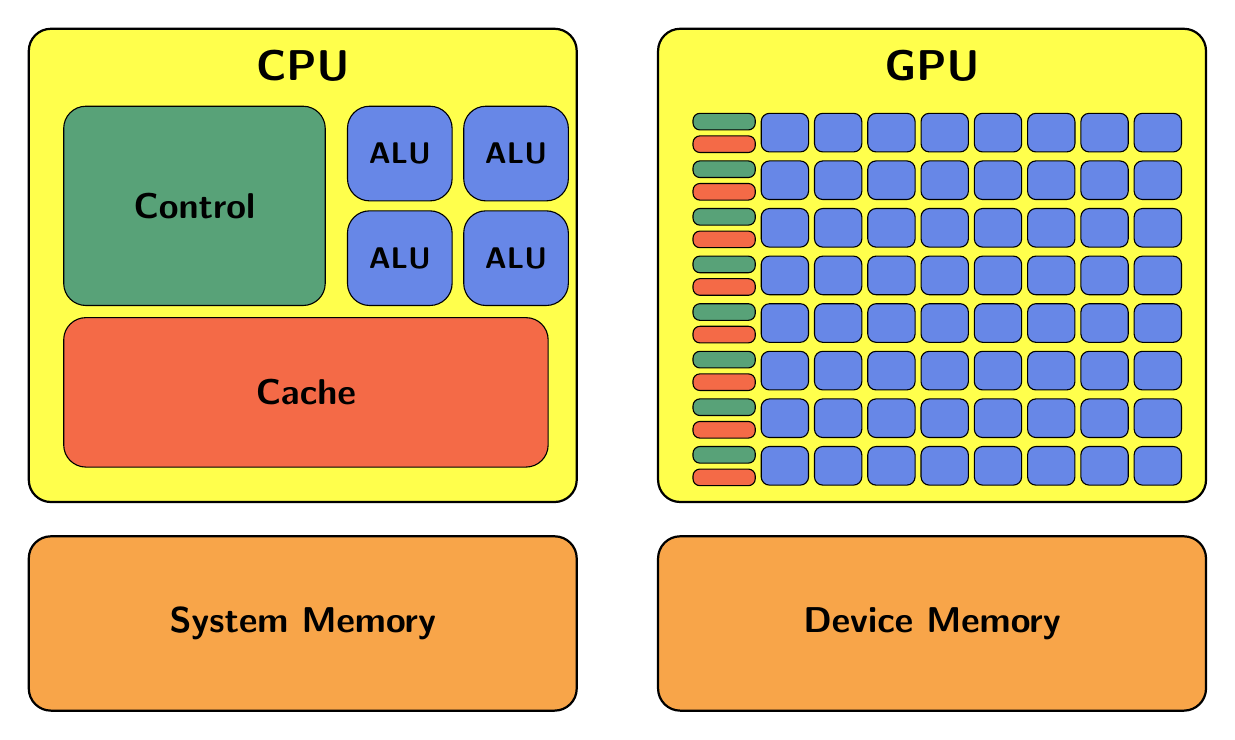
\begin{tikzpicture}[scale=0.9,transform shape]

  % Processors
  \path                       node[draw,thick,fill=Yellow!70,minimum width=22em,minimum height=19em,inner sep=0.3cm,rounded corners=8pt] (cpu) {};
  \path (cpu.east) +(5.0,0.0) node[draw,thick,fill=Yellow!70,minimum width=22em,minimum height=19em,inner sep=0.3cm,rounded corners=8pt] (gpu) {};
  \node[below] at ($(cpu.north)+(0.0,-0.2)$) {\sffamily\bfseries\LARGE{CPU}};
  \node[below] at ($(gpu.north)+(0.0,-0.2)$) {\sffamily\bfseries\LARGE{GPU}};

  % Memory
  \path (cpu.south) +(0.0,-1.7) node[draw,thick,fill=BurntOrange!70,minimum width=22em,minimum height=7em,inner sep=0.3cm,rounded corners=8pt] (cpu-memory) {\sffamily\bfseries\Large{System Memory}};
  \path (gpu.south) +(0.0,-1.7) node[draw,thick,fill=BurntOrange!70,minimum width=22em,minimum height=7em,inner sep=0.3cm,rounded corners=8pt] (gpu-memory) {\sffamily\bfseries\Large{Device Memory}};

  % CPU
  \path (cpu.north west) +(0.5,-1.1) node[anchor=north west,draw,fill=SeaGreen!80,text centered,minimum width=10.5em,minimum height=8em,inner sep=0.3cm,rounded corners=8pt] (cpu-control) {\sffamily\bfseries\Large{Control}};
  \path (cpu.south west) +(0.5,0.5) node[anchor=south west,draw,fill=RedOrange!80,text centered,minimum width=19.45em,minimum height=6em,inner sep=0.3cm,rounded corners=8pt] (cpu-cache) {\sffamily\bfseries\Large{Cache}};
  \path (cpu-control.north east) +(0.3,0.0) node[anchor=north west,draw,fill=RoyalBlue!80,text centered,minimum width=3.8em,minimum height=3.8em,inner sep=0.3cm,rounded corners=8pt] (cpu-alu-0) {\sffamily\bfseries\large{ALU}};
  \path (cpu-alu-0.north east) +(0.15,0.0) node[anchor=north west,draw,fill=RoyalBlue!80,text centered,minimum width=3.8em,minimum height=3.8em,inner sep=0.3cm,rounded corners=8pt] (cpu-alu-1) {\sffamily\bfseries\large{ALU}};
  \path (cpu-control.south east) +(0.3,0.0) node[anchor=south west,draw,fill=RoyalBlue!80,text centered,minimum width=3.8em,minimum height=3.8em,inner sep=0.3cm,rounded corners=8pt] (cpu-alu-2) {\sffamily\bfseries\large{ALU}};
  \path (cpu-alu-2.north east) +(0.15,0.0) node[anchor=north west,draw,fill=RoyalBlue!80,text centered,minimum width=3.8em,minimum height=3.8em,inner sep=0.3cm,rounded corners=8pt] (cpu-alu-3) {\sffamily\bfseries\large{ALU}};
  
  % GPU
  % \core{<id>}{<pos>}
  \DeclareDocumentCommand \core { m m }{%
    \path #2 node[anchor=north west,draw,fill=SeaGreen!80,text centered,minimum width=2.5em,minimum height=0.4em,rounded corners=2.5pt] (gpu-control-#1) {};
    \path (gpu-control-#1.south west) +(0.0,-0.07) node[anchor=north west,draw,fill=RedOrange!80,text centered,minimum width=2.5em,minimum height=0.4em,rounded corners=2.5pt] (gpu-cache-#1) {};
    \path (gpu-control-#1.north east) +(0.07,0.0) node[anchor=north west,draw,fill=RoyalBlue!80,text centered,minimum width=1.9em,minimum height=1.55em,rounded corners=3pt] (gpu-alu-#1-0) {};
    \path (gpu-alu-#1-0.north east) +(0.07,0.0) node[anchor=north west,draw,fill=RoyalBlue!80,text centered,minimum width=1.9em,minimum height=1.55em,rounded corners=3pt] (gpu-alu-#1-1) {};
    \path (gpu-alu-#1-1.north east) +(0.07,0.0) node[anchor=north west,draw,fill=RoyalBlue!80,text centered,minimum width=1.9em,minimum height=1.55em,rounded corners=3pt] (gpu-alu-#1-2) {};
    \path (gpu-alu-#1-2.north east) +(0.07,0.0) node[anchor=north west,draw,fill=RoyalBlue!80,text centered,minimum width=1.9em,minimum height=1.55em,rounded corners=3pt] (gpu-alu-#1-3) {};
    \path (gpu-alu-#1-3.north east) +(0.07,0.0) node[anchor=north west,draw,fill=RoyalBlue!80,text centered,minimum width=1.9em,minimum height=1.55em,rounded corners=3pt] (gpu-alu-#1-4) {};
    \path (gpu-alu-#1-4.north east) +(0.07,0.0) node[anchor=north west,draw,fill=RoyalBlue!80,text centered,minimum width=1.9em,minimum height=1.55em,rounded corners=3pt] (gpu-alu-#1-5) {};
    \path (gpu-alu-#1-5.north east) +(0.07,0.0) node[anchor=north west,draw,fill=RoyalBlue!80,text centered,minimum width=1.9em,minimum height=1.55em,rounded corners=3pt] (gpu-alu-#1-6) {};
    \path (gpu-alu-#1-6.north east) +(0.07,0.0) node[anchor=north west,draw,fill=RoyalBlue!80,text centered,minimum width=1.9em,minimum height=1.55em,rounded corners=3pt] (gpu-alu-#1-7) {};
  }
  \core{0}{($(gpu.north west)+(0.5,-1.2)$)}
  \core{1}{($(gpu-cache-0.south west)+(0.0,-0.105)$)}
  \core{2}{($(gpu-cache-1.south west)+(0.0,-0.105)$)}
  \core{3}{($(gpu-cache-2.south west)+(0.0,-0.105)$)}
  \core{4}{($(gpu-cache-3.south west)+(0.0,-0.105)$)}
  \core{5}{($(gpu-cache-4.south west)+(0.0,-0.105)$)}
  \core{6}{($(gpu-cache-5.south west)+(0.0,-0.105)$)}
  \core{7}{($(gpu-cache-6.south west)+(0.0,-0.105)$)}

\end{tikzpicture}
\caption{CPU and GPU architectures.}
\label{fig:processor-architectures}
\end{figure}

\clearpage
%!TEX root = ../main.tex

\begin{figure}[p]
\centering
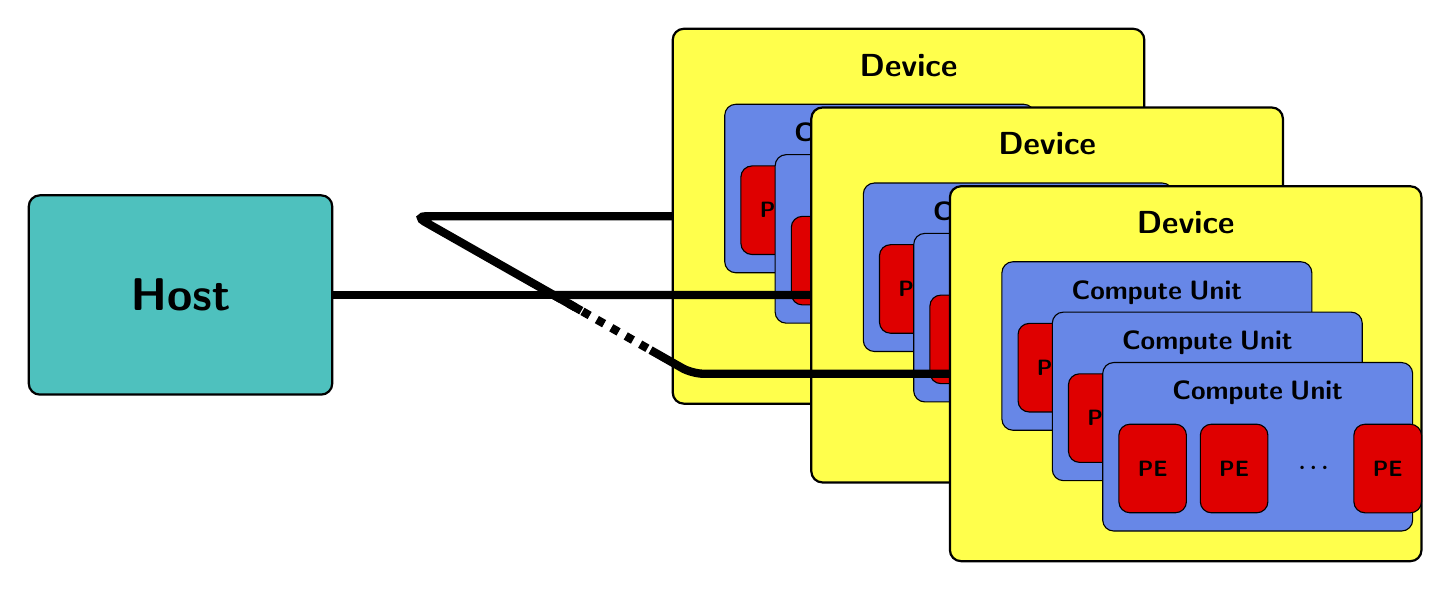
\begin{tikzpicture}[scale=0.8,transform shape]

  % Parameters
  \def\pesep{0.75}

  % Styles
  \tikzstyle{every node}=[draw,rounded corners,text centered]
  \tikzstyle{host}=[thick,fill=TealBlue!80,text width=12em,minimum width=12em,minimum height=9em,inner sep=0.3cm]
  \tikzstyle{dev}=[thick,fill=Yellow!70,text width=12em,minimum width=21.3em,inner sep=0.4cm]
  \tikzstyle{unit}=[fill=RoyalBlue!80,text width=12em,minimum width=14em,inner sep=0.3cm]
  \tikzstyle{pe}=[fill=Maroon!25!Red,minimum width=2em,minimum height=4em,inner sep=0.3cm]
  \tikzstyle{line}=[line width=3pt,rounded corners]

  % \<dev/unit/pe>{<id>}{<label>}
  \newcommand{\dev}[2]{node[dev] (#1) {\sffamily\bfseries\Large{#2}}}
  \newcommand{\unit}[2]{node[unit] (#1) {\sffamily\bfseries\large{#2}}}
  \newcommand{\pe}[2]{node[pe] (#1) {\sffamily\bfseries{#2}}}
  
  % \cunit{<id>}{<origin>}{<shift>}
  \newcommand{\cunit}[3]{%
    \path[shift={#3}] ($#2+(3.3,-2.55)$) \unit{compute-unit-#1-0}{Compute Unit\vspace{1.7cm}};
    \path[shift={#3}] (compute-unit-#1-0.south west) +(0.8,1.0)  \pe{pe-#1-0}{PE};
    \path[shift={#3}] (pe-#1-0.east)+(\pesep,0) \pe{pe-#1-1}{PE};
    \node[draw=none] (dots-#1-0) at ($(pe-#1-1.east)+(\pesep,0)$) {$\bm\cdots$};
    \path (dots-#1-0.east)+(\pesep,0) \pe{pe-#1-2}{PE};
  }

  % \cdev{<id>}{<shift>}
  \newcommand{\cdev}[2]{%
    \path[shift={#2}] (0,0) \dev{dev-#1}{Device\vspace{4.8cm}};
    \cunit{#1-0}{($(dev-#1.north west)+(0.0, 0.0)$)}{#2}
    \cunit{#1-1}{($(dev-#1.north west)+(0.8,-0.8)$)}{#2}
    \cunit{#1-2}{($(dev-#1.north west)+(1.6,-1.6)$)}{#2}
  }

  % ===========================================================================
 
  % Draw devices
  \cdev{0}{(0.0, 0.0 )}
  \cdev{1}{(2.2,-1.25)}
  \cdev{2}{(4.4,-2.5 )}

  % Draw host
  \node[host] (host) at ($(dev-1.west)+(-10.0,0.0)$) {\sffamily\bfseries\huge{Host}};
    
  % Draw interconnect
  \draw[line] (host.east) -- ++(3.5,0.0);
  \draw[line] ($(host.east)+(3.5,0.0)$) -- ++(-2.2,1.25) -- (dev-0.west);
  \draw[line] ($(host.east)+(3.5,0.0)$) -- (dev-1.west);
  \draw[line] ($(host.east)+(3.5,0.0)$) -- ++($0.2*(2.2,-1.25)$);
  \draw[line,dashed] ($(host.east)+(3.5,0.0)$) -- ++($0.7*(2.2,-1.25)$);
  \draw[line] ($(host.east)+(3.5,0.0)+0.7*(2.2,-1.25)$) -- ($(host.east)+(3.5,0.0)+(2.2,-1.25)$) -- (dev-2.west);

\end{tikzpicture}
\caption{OpenCL abstract hardware model.}
\label{fig:hardware-model}
\end{figure}

\clearpage
%!TEX root = ../main.tex

\begin{figure}[p]
\centering
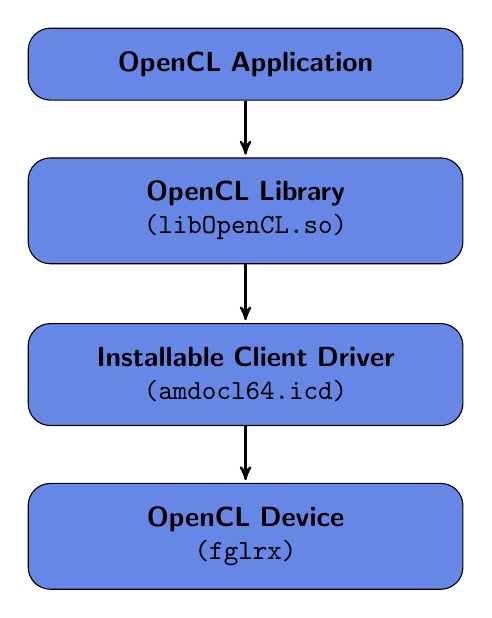
\begin{tikzpicture}[scale=1.0,transform shape]

  % Styles
  \tikzstyle{block}=[draw,fill=RoyalBlue!80,text centered,text width=14em,minimum width=14em,inner sep=0.3cm,rounded corners=8pt]
  \tikzstyle{to}=[->,>=stealth',shorten >=1pt,thick]

  % \block{<id>}{<label>}
  \newcommand{\block}[2]{node[block] (#1) {\sffamily\bfseries{#2}}}

  % ===========================================================================
 
  % Draw blocks
  \path                         \block{app}{OpenCL Application};
  \path (app.south) +(0.0,-1.4) \block{lib}{OpenCL Library\\\ttfamily(libOpenCL.so)};
  \path (lib.south) +(0.0,-1.4) \block{icd}{Installable Client Driver\\\ttfamily(amdocl64.icd)};
  \path (icd.south) +(0.0,-1.4) \block{dev}{OpenCL Device\\\ttfamily(fglrx)};
    
  % Draw arrows
  \draw[to] (app.south) -- (lib.north);
  \draw[to] (lib.south) -- (icd.north);
  \draw[to] (icd.south) -- (dev.north);

\end{tikzpicture}
\caption{Data flow diagram for an OpenCL application.}
\label{fig:dfd-opencl-app}
\end{figure}

\clearpage
%!TEX root = ../main.tex

\begin{figure}[p]
\centering
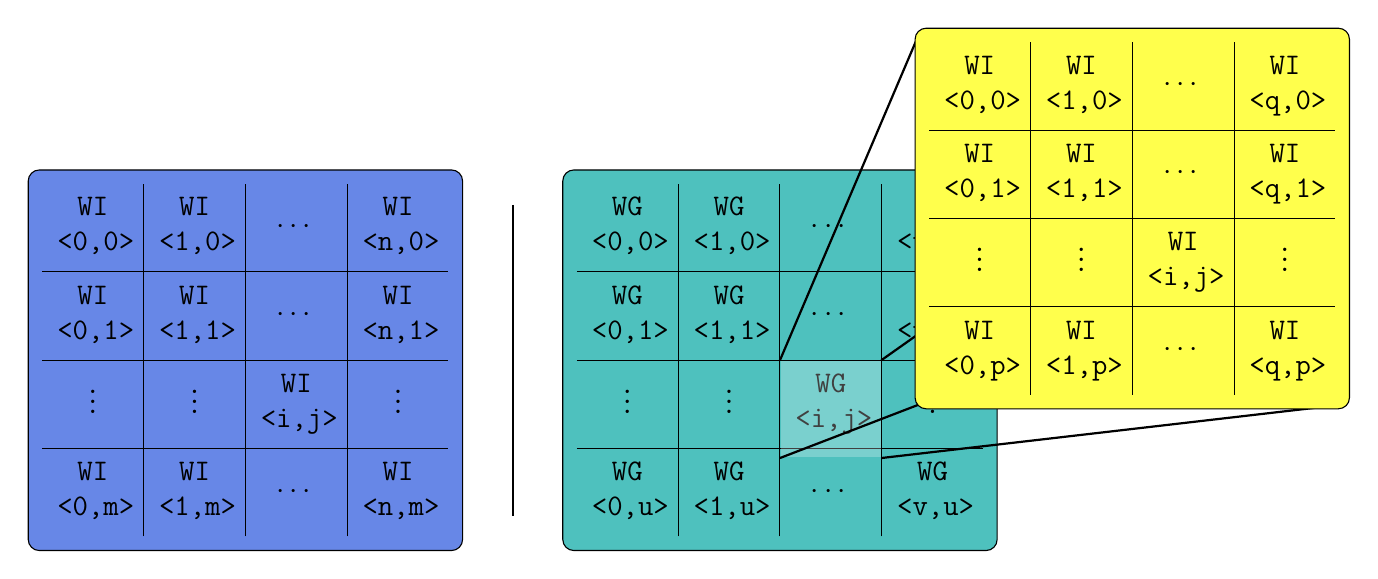
\begin{tikzpicture}[scale=0.9,transform shape]

  % Parameters
  \renewcommand{\arraystretch}{2.3} 
  \setlength{\extrarowheight}{-1mm} 

  % Layers
  \pgfdeclarelayer{front-0}
  \pgfdeclarelayer{front-1}
  \pgfsetlayers{main,front-0,front-1}

  % \is{<id>}{<pos>}{<label>}{<x-limit>}{<y-limit>}{<background-color>}
  \DeclareDocumentCommand \is { m m m m m m }{%
    \node[anchor=west,draw,rounded corners,fill=#6,inner sep=0.2cm] (wi-#1) at #2 {%
    \begin{tabular}{ >{\centering\arraybackslash\ttfamily\bfseries\large} m{1cm} | 
                     >{\centering\arraybackslash\ttfamily\bfseries\large} m{1cm} | 
                     >{\centering\arraybackslash\ttfamily\bfseries\large} m{1cm} | 
                     >{\centering\arraybackslash\ttfamily\bfseries\large} m{1cm} } 
      #3\linebreak<0,0>  & #3\linebreak<1,0>  & $\cdots$          & #3\linebreak<#4,0>  \\\hline
      #3\linebreak<0,1>  & #3\linebreak<1,1>  & $\cdots$          & #3\linebreak<#4,1>  \\\hline
      $\vdots$           & $\vdots$           & #3\linebreak<i,j> & $\vdots$            \\\hline
      #3\linebreak<0,#5> & #3\linebreak<1,#5> & $\cdots$          & #3\linebreak<#4,#5> \\
    \end{tabular}
    };
  }

  % ===========================================================================

  % Index spaces
  \is{0}{(0,0)}{WI}{n}{m}{RoyalBlue!80}
  \is{1}{($(wi-0.east)+(1.4,0)$)}{WG}{v}{u}{TealBlue!80}  
  \begin{pgfonlayer}{front-1}
  \is{2}{($(wi-1)+(1.9,2.0)$)}{WI}{q}{p}{Yellow!70}
  \end{pgfonlayer}

  % Separating line
  \draw[thick] ($(wi-0.north east)+(0.7,-0.5)$) -- ($(wi-0.south east)+(0.7,0.5)$);

  % Zoom lines
  \begin{pgfonlayer}{front-0}
  \draw[thick] ($(wi-1)+(-0.00,-0.00)$) node (wi-tl) {} -- ($(wi-2.north west)+( 0.07,-0.07)$);
  \draw[thick] ($(wi-1)+( 1.43,-0.00)$) -- ($(wi-2.north east)+(-0.07,-0.07)$);
  \draw[thick] ($(wi-1)+( 0.00,-1.38)$) -- ($(wi-2.south west)+( 0.07, 0.07)$);
  \draw[thick] ($(wi-1)+( 1.43,-1.38)$) node (wi-br) {} -- ($(wi-2.south east)+(-0.07, 0.07)$);
  \end{pgfonlayer}

  % Shade
  \draw[draw=none,fill=white,opacity=0.25] ($(wi-tl)+(0.01,-0.01)$) rectangle ($(wi-br)+(-0.01,0.01)$);

\end{tikzpicture}
\caption{Index space during a kernel execution. This space is further divided into groups.}
\label{fig:index-spaces}
\end{figure}

\clearpage
%!TEX root = ../main.tex

\begin{figure}[p]
\centering
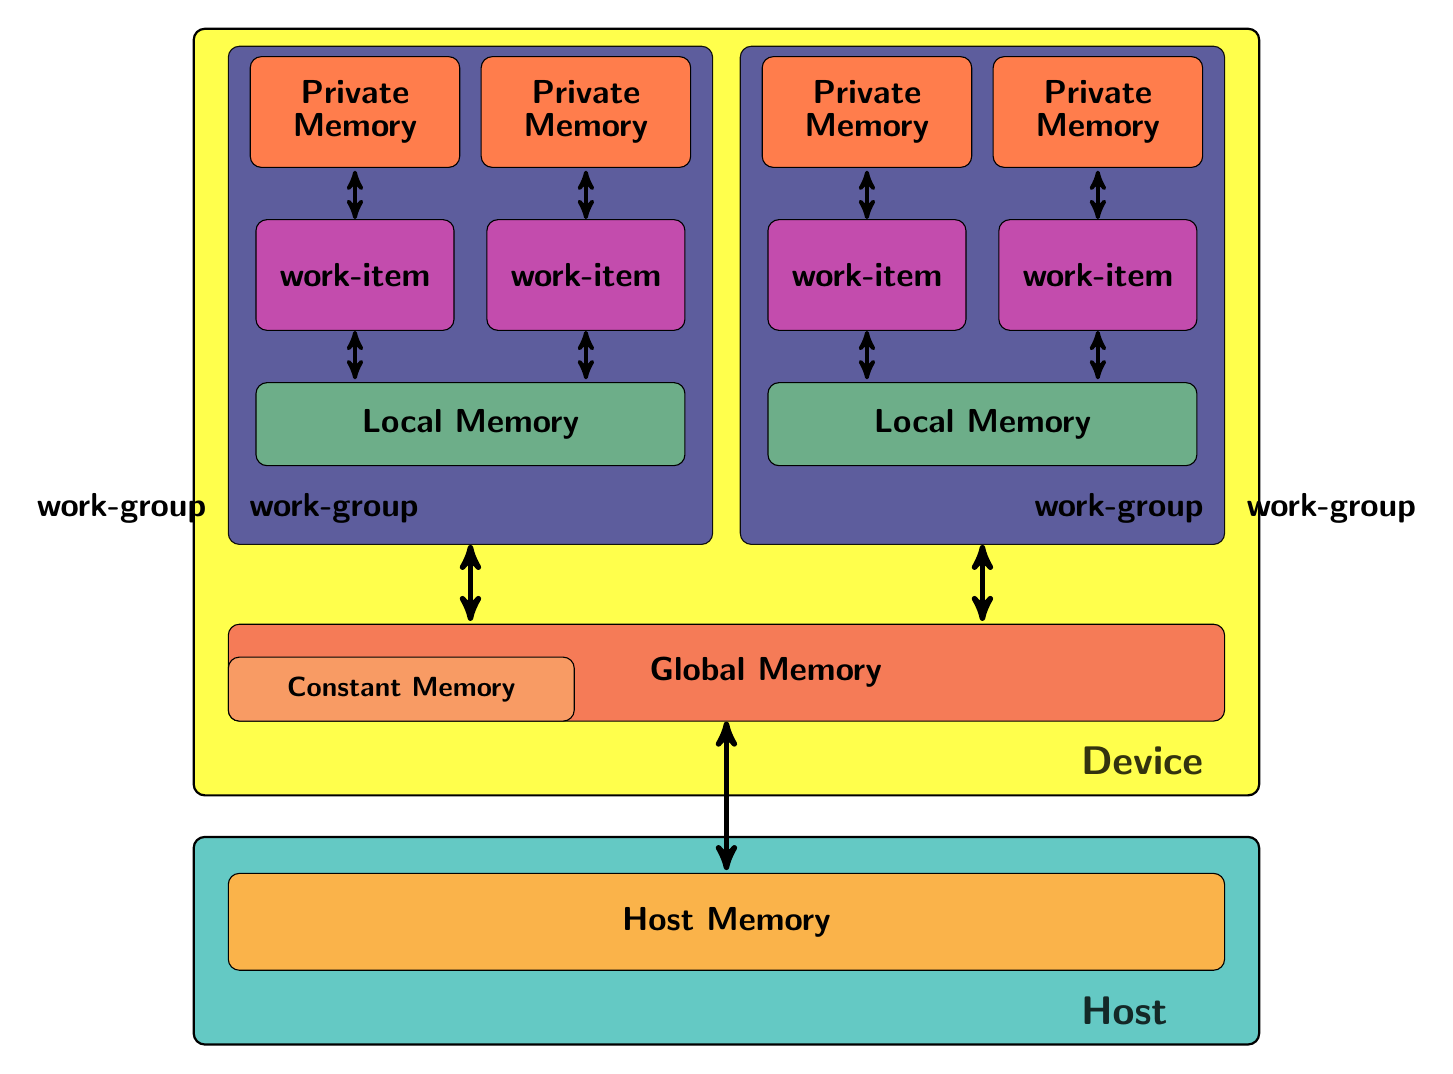
\begin{tikzpicture}[scale=1.0,transform shape]

  % Styles
  \tikzstyle{every node}=[draw,rounded corners,text centered]
  \tikzstyle{host}=[thick,fill=TealBlue!70,minimum width=38.5em,minimum height=7.5em,inner sep=0.3cm]
  \tikzstyle{dev}=[thick,fill=Yellow!70,minimum width=38.5em,minimum height=27.7em,inner sep=0.3cm]
  \tikzstyle{ram}=[text centered,minimum width=36em,minimum height=3.5em,inner sep=0.3cm]
  \tikzstyle{constant}=[fill=Peach!80,text centered,minimum width=12.5em,minimum height=2em,inner xsep=0.3cm,inner ysep=0.25cm]
  \tikzstyle{group}=[fill=NavyBlue!70,minimum width=17.5em,minimum height=18em,inner sep=0.3cm]
  \tikzstyle{local}=[fill=SeaGreen!70,minimum width=15.5em,minimum height=3em,inner sep=0.3cm]
  \tikzstyle{wi}=[fill=RoyalPurple!30!CarnationPink,minimum width=7em,minimum height=4em,inner sep=0.3cm]
  \tikzstyle{private}=[fill=OrangeRed!70,text width=7em,minimum width=6em,minimum height=4em,inner xsep=0.1cm,inner ysep=0.3cm]
  \tikzstyle{bus}=[<->,>=stealth',shorten >=1pt,line width=2.0pt]
  \tikzstyle{bus2}=[<->,>=stealth',shorten >=1pt,line width=1.4pt]
  \tikzstyle{label}=[draw=none]

  % \memory{<id>}{<pos>}{<color>}{<label>}
  \DeclareDocumentCommand \memory { m m m m }{\path #2 node[ram,anchor=south,fill=#3] (#1) {\sffamily\bfseries\large{#4}};}

  % \group{<id>}{<pos>}{<anchor}
  \DeclareDocumentCommand \group { m m m }{%
    \path #2 node[group,anchor=#3,opacity=0.9] (#1) {};
    \ifthenelse{\equal{#3}{south west}}%
    {\node[label,above right] at ($(#1.#3)+(0.15,0.15)$) {\sffamily\bfseries\large{work-group}};}%
    {\node[label,above left] at ($(#1.#3)+(-0.15,0.15)$) {\sffamily\bfseries\large{work-group}};}
  }

  % \content{<id>}{<pos>}
  \DeclareDocumentCommand \content { m m }{%
    \path #2 node[local,anchor=south] (local-#1) {\sffamily\bfseries\large{Local Memory}};
    \path (local-#1.north west)+(0.0,0.65) node[wi,anchor=south west] (wi-#1-0) {\sffamily\bfseries\large{work-item}};
    \path (local-#1.north east)+(0.0,0.65) node[wi,anchor=south east] (wi-#1-1) {\sffamily\bfseries\large{work-item}};
    \draw[bus2] (wi-#1-0.south) -- (wi-#1-0.south |- local-#1.north);
    \draw[bus2] (wi-#1-1.south) -- (wi-#1-1.south |- local-#1.north);
    \path (wi-#1-0.north)+(0.0,0.65) node[private,anchor=south] (private-#1-0) {\sffamily\bfseries\large{Private Memory}};
    \path (wi-#1-1.north)+(0.0,0.65) node[private,anchor=south] (private-#1-1) {\sffamily\bfseries\large{Private Memory}};
    \draw[bus2] (wi-#1-0.north) -- (private-#1-0.south);
    \draw[bus2] (wi-#1-1.north) -- (private-#1-1.south);
  }

  % ===========================================================================
 
  % Draw device
  \path node[dev] (dev) {};
  \node[label,above right,opacity=0.8] at ($(dev.south east)+(-2.4,0.15)$) {\sffamily\bfseries\Large{Device}};
  \memory{global-mem}{($(dev.south)+(0.0,0.95)$)}{RedOrange!70}{{\hspace{1cm}Global Memory}}
  \path (global-mem.south west) node[constant,anchor=south west] (constant) {\sffamily\bfseries{Constant Memory}};
  \group{group-0}{($(global-mem.north west)+(0.0,1.0)$)}{south west}
  \group{group-1}{($(global-mem.north east)+(0.0,1.0)$)}{south east}
  \content{0}{($(group-0.south)+(0.0,1.0)$)}
  \content{1}{($(group-1.south)+(0.0,1.0)$)}
  
  % Draw host
  \path (dev.south)+(0.0,-0.5) node[host,anchor=north] (host) {};
  \node[label,above right,opacity=0.8] at ($(host.south east)+(-2.4,0.15)$) {\sffamily\bfseries\Large{Host}};
  \memory{host-mem}{($(host.south)+(0.0,0.95)$)}{YellowOrange!70}{Host Memory}

  % Draw arrows
  \draw[bus] (global-mem.south) -- (host-mem.north);
  \draw[bus] (group-0.south) -- (group-0.south |- global-mem.north);
  \draw[bus] (group-1.south) -- (group-1.south |- global-mem.north);

\end{tikzpicture}
\caption{OpenCL abstract memory model.}
\label{fig:memory-model}
\end{figure}

\clearpage
%!TEX root = ../main.tex

\begin{figure}[p]
\centering
\hspace*{-1.5cm}
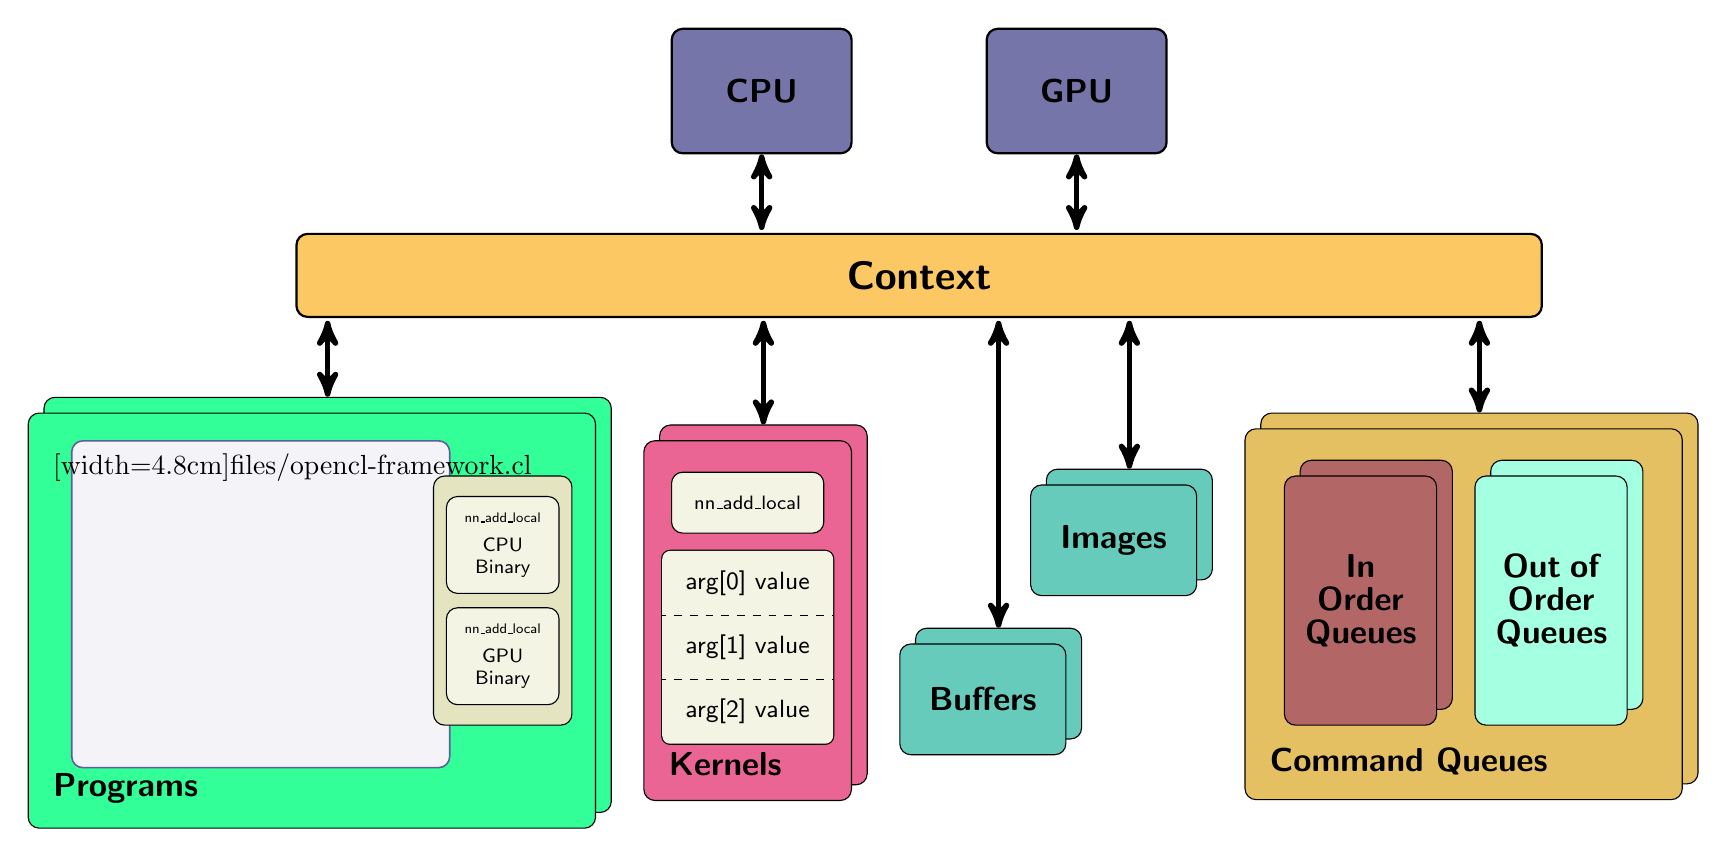
\begin{tikzpicture}[scale=1.0,transform shape]
  
  % Styles
  \tikzstyle{every node}=[draw,rounded corners,text centered]
  \tikzstyle{context}=[thick,fill=Dandelion!70,minimum width=45em,minimum height=3em,inner sep=0.3cm]
  \tikzstyle{processor}=[thick,fill=MidnightBlue!60,minimum width=6.5em,minimum height=4.5em,inner sep=0.3cm]
  \tikzstyle{program}=[fill=SpringGreen!80,minimum width=20.5em,minimum height=15.0em,inner sep=0.3cm]
  \tikzstyle{source}=[draw=MidnightBlue!70,fill=MidnightBlue!5,minimum width=4.8cm,minimum height=4.15cm,line width=0.2mm,inner sep=0.3cm]
  \tikzstyle{binary-frame}=[fill=Gray!60!Yellow!35!White,minimum width=5em,minimum height=9em,inner sep=0.3cm]
  \tikzstyle{binary}=[fill=Gray!60!Yellow!15!White,text width=3.5em,minimum width=4em,minimum height=3.5em,inner sep=0.1cm]
  \tikzstyle{kernel-frame}=[fill=WildStrawberry!60!Orchid!80!White,minimum width=7.5em,minimum height=13.0em,inner sep=0.3cm]
  \tikzstyle{kernel-name}=[fill=Gray!60!Yellow!15!White,minimum width=5.5em,minimum height=2.2em,inner xsep=0cm,inner ysep=0.1cm]
  \tikzstyle{memory}=[fill=Emerald!60,minimum width=6em,minimum height=4em,inner sep=0.3cm]
  \tikzstyle{queue-frame}=[fill=Goldenrod!70,minimum width=15.8em,minimum height=13.4em,inner sep=0.3cm]
  \tikzstyle{queue}=[text width=4em,minimum width=5.5em,minimum height=9.0em,inner sep=0cm]
  \tikzstyle{bus}=[<->,>=stealth',shorten >=1pt,line width=2.0pt]

  % ===========================================================================
 
  % Context
  \path node[context] (context) {\sffamily\bfseries\Large{Context}};
  % Processors
  \path (context.north)+(-2.0,1.8) node[processor] (cpu) {\sffamily\bfseries\large{CPU}};
  \path (context.north)+(2.0,1.8) node[processor] (gpu) {\sffamily\bfseries\large{GPU}};
  % Programs
  \path (context.south west)+(-3.2,-1.0) node[program,anchor=north west] (program-0) {};
  \path (program-0)+(-0.2,-0.2) node[program] (program-1) {};
  \node[draw=none,anchor=south west] at ($(program-1.south west)+(0.2,0.2)$) {\sffamily\bfseries\large{Programs}};
  \path (program-1.north west)+(0.55,-0.35) node[source,anchor=north west] (source-0) {};
  \node[draw=none,anchor=north west] (source-1) at ($(program-1.north west)+(0.2,-0.4)$) {\mycodembed[width=4.8cm]{files/opencl-framework.cl}};
  \path (program-1.north east)+(-0.3,-0.8) node[binary-frame,anchor=north east] (binary-frame) {};
  \path (binary-frame.north)+(0.0,-0.26) node[binary,anchor=north] (binary-0) {\sffamily\tiny\baselineskip=0mm nn\_add\_local\vspace{0.8mm} \scriptsize CPU Binary \par};
  \path (binary-frame.south)+(0.0,0.26) node[binary,anchor=south] (binary-1) {\sffamily\tiny\baselineskip=0mm nn\_add\_local\vspace{0.8mm} \scriptsize GPU Binary \par};
  % Kernels
  \path (program-0.east)+(0.6,0.0) node[kernel-frame,anchor=west] (kernel-0) {};
  \path (kernel-0)+(-0.2,-0.2) node[kernel-frame] (kernel-1) {};
  \node[draw=none,anchor=south west] at ($(kernel-1.south west)+(0.2,0.2)$) {\sffamily\bfseries\large{Kernels}};
  \path (kernel-1.north)+(0.0,-0.4) node[kernel-name,anchor=north] (kernel-name) {\sffamily\scriptsize nn\_add\_local};
  \path (kernel-name.south)+(0.0,-0.08) node[draw=none,anchor=north] (kernel-args) {\begin{tcolorbox}[colback=Gray!60!Yellow!15!White,colframe=black,fontupper=\sffamily\small,right=0mm,left=0mm,boxsep=0.5mm,boxrule=0.15mm,width=2.2cm,halign=center] arg[0] value\tcbline arg[1] value\tcbline arg[2] value\end{tcolorbox}};
  % Memory objects
  \path (kernel-0.east)+(0.6,-1.0) node[memory,anchor=west] (buffer-0) {};
  \path (buffer-0)+(-0.2,-0.2) node[memory] (buffer-1) {\sffamily\bfseries\large{Buffers}};
  \path (buffer-0.north)+(0.6,0.6) node[memory,anchor=south west] (image-0) {};
  \path (image-0)+(-0.2,-0.2) node[memory] (image-1) {\sffamily\bfseries\large{Images}};
  % Command queues
  \path (program-0.north -| image-0.east)+(0.6,-0.2) node[queue-frame,anchor=north west] (queue-frame-0) {};
  \path (queue-frame-0)+(-0.2,-0.2) node[queue-frame] (queue-frame-1) {};
  \node[draw=none,anchor=south west] at ($(queue-frame-1.south west)+(0.2,0.2)$) {\sffamily\bfseries\large{Command Queues}};
  \path (queue-frame-1.north west)+(0.7,-0.4) node[queue,anchor=north west,fill=Maroon!60] (queue-in-0) {};
  \path (queue-in-0)+(-0.2,-0.2) node[queue,fill=Maroon!60] (queue-in-1) {\sffamily\bfseries\large{In Order Queues}};
  \path (queue-frame-1.north east)+(-0.5,-0.4) node[queue,anchor=north east,fill=Aquamarine!70] (queue-out-0) {};
  \path (queue-out-0)+(-0.2,-0.2) node[queue,fill=Aquamarine!70] (queue-out-1) {\sffamily\bfseries\large{Out of Order Queues}};

  % Draw connections
  \draw[bus] (cpu) -- (cpu |- context.north);
  \draw[bus] (gpu) -- (gpu |- context.north);
  \draw[bus] (program-0.north) -- (program-0.north |- context.south);
  \draw[bus] (kernel-0.north) -- (kernel-0.north |- context.south);
  \draw[bus] (buffer-0.north) -- (buffer-0.north |- context.south);
  \draw[bus] (image-0.north) -- (image-0.north |- context.south);
  \draw[bus] (queue-frame-0.north) -- (queue-frame-0.north |- context.south);

\end{tikzpicture}
\caption{OpenCL framework.}
\label{fig:opencl-framework}
\end{figure}

\clearpage
%!TEX root = ../main.tex

\begin{figure}[p]
\centering
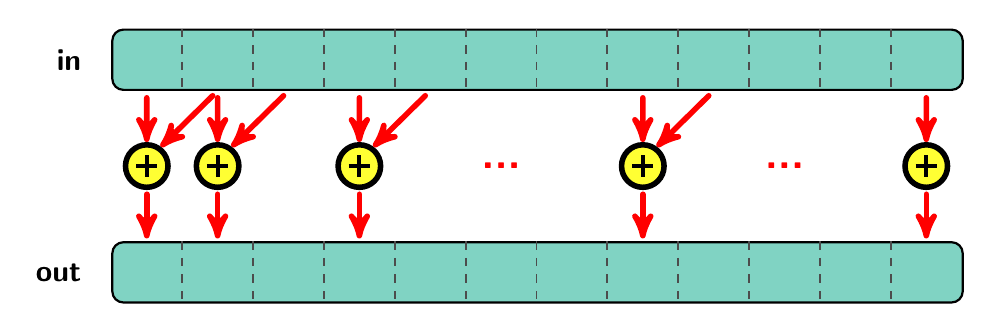
\begin{tikzpicture}[scale=0.9,transform shape]

  % Parameters
  \def\xcell{1.0cm}
  \def\ycell{8.5mm}
  \def\radius{0.3cm}

  % Styles
  \tikzstyle{table}=[draw,anchor=north west,thick,rounded corners]
  \tikzstyle{line}=[dashed,line width=0.7pt]
  \tikzstyle{to}=[->,>=stealth',shorten <=2.5pt,shorten >=1pt,line width=2.0pt,red,cap=round]

  % \table*{<id>}{<pos>}{<x-dim>}{<y-dim>}{<cell-lalbel-list>}[<optional-arguments>]
  % The star (*) argument enables drawing of lines between the cells
  \DeclareDocumentCommand \table { s m m m m m O{} }{%
    \path #3 node[table,minimum width=#4*\xcell,minimum height=#5*\ycell,#7] (table-#2) {};
    \IfBooleanT{#1}{%
      \pgfmathsetmacro\xdim{#4-1}
      \pgfmathsetmacro\ydim{#5-1}
      \ifnumgreater{#5}{1}{%
        \foreach \y in {1,...,\ydim}
          \draw[line,Black!70] ($(table-#2.north west)+(0,-\y*\ycell)$) -- ++(#4*\xcell,0);}{}
      \ifnumgreater{#4}{1}{%
        \foreach \x in {1,...,\xdim}
          \draw[line,Black!70] ($(table-#2.north west)+(\x*\xcell,0)$) -- ++(0,-#5*\ycell);}{}
    }
    \foreach[count=\li from 0] \l in {#6}{%
      \pgfmathsetmacro\lx{mod(\li,#4) + 0.5}
      \pgfmathsetmacro\ly{int(\li/#4) + 0.5}
      \node (cell-label-#2-\li) at ($(table-#2.north west)+(\lx*\xcell,-\ly*\ycell)$) {\l};
    }
  }

  % \adder*{<x-offset>}
  % The star (*) argument disables drawing of the second adder argument arrow
  \DeclareDocumentCommand \adder { s m }{%
    \node (mid-dist) at ($(table-0.south west)!0.5!(table-1.north west)+(#2,0)$) {};
    \draw[line width=2pt,fill=Yellow!80] (mid-dist) circle (\radius);
    \draw[line width=1.5pt] ($(mid-dist)+(180:\radius-1.5mm)$) -- ($(mid-dist)+(0:\radius-1.5mm)$);
    \draw[line width=1.5pt] ($(mid-dist)+(-90:\radius-1.5mm)$) -- ($(mid-dist)+(90:\radius-1.5mm)$);
    \draw[to] ($(table-0.south west)+(#2,0)$) -- ($(mid-dist)+(0,\radius)$);
    \draw[to] ($(mid-dist)+(0,-\radius)$) -- (mid-dist |- table-1.north);
    \IfBooleanF{#1}{%
      \draw[to] ($(table-0.south west)+({#2+\xcell},0)$) -- ($(mid-dist)+(55:\radius)$);}
  }

  % ===========================================================================
 
  % Draw tables
  \table*{0}{(0.0, 0.0)}{12}{1}{}[fill=Emerald!50]
  \table*{1}{(0.0,-3.0)}{12}{1}{}[fill=Emerald!50]

  % Draw labels
  \node[anchor=east] at ($(table-0.west)+(-0.3,0.0)$) {\sffamily\bfseries\large{in}};
  \node[anchor=east] at ($(table-1.west)+(-0.3,0.0)$) {\sffamily\bfseries\large{out}};

  % Draw adders
  \adder{0.5*\xcell}
  \adder{1.5*\xcell}
  \adder{3.5*\xcell}
  \adder{7.5*\xcell}
  \node[red] at ($(table-0.south west)!0.5!(table-1.north west)+(5.5,0)$) {\sffamily\bfseries\LARGE{...}};
  \node[red] at ($(table-0.south west)!0.5!(table-1.north west)+(9.5,0)$) {\sffamily\bfseries\LARGE{...}};
  \adder*{11.5*\xcell}

\end{tikzpicture}
\caption{{\ttfamily nn\_add}: Every output element is the sum of the corresponding input element and its next element.}
\label{fig:nn-add}
\end{figure}

\clearpage
%!TEX root = ../main.tex

\begin{figure}[p]
\centering
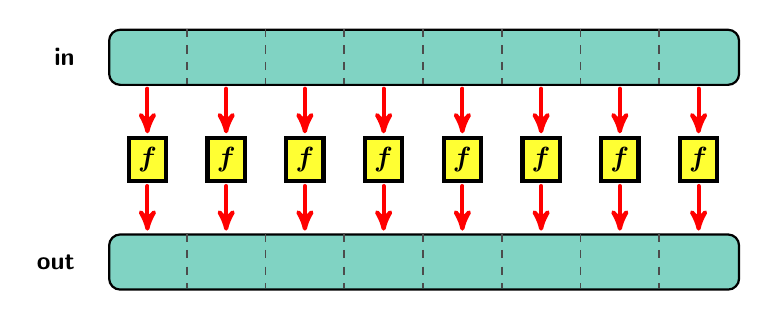
\begin{tikzpicture}[scale=1.0,transform shape]

  % Parameters
  \def\xcell{1.0cm}
  \def\ycell{0.7cm}

  % Styles
  \tikzstyle{table}=[draw,anchor=north west,thick,rounded corners]
  \tikzstyle{line}=[dashed,line width=0.7pt]
  \tikzstyle{to}=[->,>=stealth',shorten <=1pt,shorten >=1pt,line width=1.5pt,red,cap=round]

  % \table*{<id>}{<pos>}{<x-dim>}{<y-dim>}{<cell-lalbel-list>}[<optional-arguments>]
  % The star (*) argument enables drawing of lines between the cells
  \DeclareDocumentCommand \table { s m m m m m O{} }{%
    \path #3 node[table,minimum width=#4*\xcell,minimum height=#5*\ycell,#7] (table-#2) {};
    \IfBooleanT{#1}{%
      \pgfmathsetmacro\xdim{#4-1}
      \pgfmathsetmacro\ydim{#5-1}
      \ifnumgreater{#5}{1}{%
        \foreach \y in {1,...,\ydim}
          \draw[line,Black!70] ($(table-#2.north west)+(0,-\y*\ycell)$) -- ++(#4*\xcell,0);}{}
      \ifnumgreater{#4}{1}{%
        \foreach \x in {1,...,\xdim}
          \draw[line,Black!70] ($(table-#2.north west)+(\x*\xcell,0)$) -- ++(0,-#5*\ycell);}{}
    }
    \foreach[count=\li from 0] \l in {#6}{%
      \pgfmathsetmacro\lx{mod(\li,#4) + 0.5}
      \pgfmathsetmacro\ly{int(\li/#4) + 0.5}
      \node (cell-label-#2-\li) at ($(table-#2.north west)+(\lx*\xcell,-\ly*\ycell)$) {\l};
    }
  }

  % \adder{<top-table-id>}{<bottom-table-id>}{<x-offset>}
  \DeclareDocumentCommand \adder { m m m }{%
    \path ($(table-#1.south west)!0.5!(table-#2.north west)+(#3,0)$) node[draw,line width=1.5pt,fill=Yellow!80,minimum width=4mm,minimum height=4mm] (mid-dist) {$\bm f$};
    \draw[to] ($(table-#1.south west)+(#3,0)$) -- (mid-dist.north);
    \draw[to] (mid-dist.south) -- (mid-dist |- table-#2.north);
  }

  % ===========================================================================
 
  % Draw tables
  \table*{0}{(0.0, 0.0)}{8}{1}{}[fill=Emerald!50]
  \table*{1}{(0.0,-2.6)}{8}{1}{}[fill=Emerald!50]

  % Draw labels
  \node[anchor=east] at ($(table-0.west)+(-0.3,0.0)$) {\sffamily\bfseries\small{in}};
  \node[anchor=east] at ($(table-1.west)+(-0.3,0.0)$) {\sffamily\bfseries\small{out}};

  % Draw adders  
  \foreach \x in {0,1,...,7}{%
    \pgfmathsetmacro\offset{\x + 0.5}
    \adder{0}{1}{\offset*\xcell}
  }

\end{tikzpicture}
\caption{Representation of map.}
\label{fig:map}
\end{figure}

\clearpage
%!TEX root = ../main.tex

\begin{figure}[p]
\centering
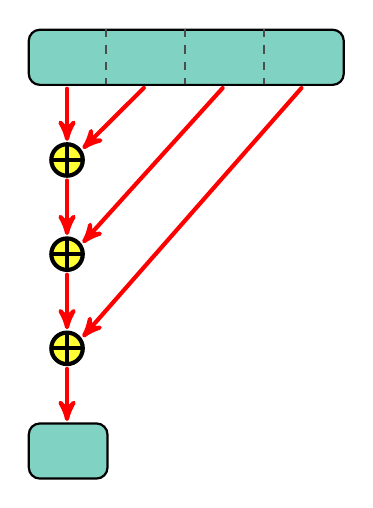
\begin{tikzpicture}[scale=1.0,transform shape]

  % Parameters
  \def\xcell{1.0cm}
  \def\ycell{0.7cm}
  \def\radius{0.2cm}

  % Styles
  \tikzstyle{table}=[draw,anchor=north west,thick,rounded corners]
  \tikzstyle{line}=[dashed,line width=0.7pt]
  \tikzstyle{to}=[->,>=stealth',shorten <=1pt,shorten >=0.5pt,line width=1.5pt,red,cap=round]

  % \table*{<id>}{<pos>}{<x-dim>}{<y-dim>}{<cell-lalbel-list>}[<optional-arguments>]
  % The star (*) argument enables drawing of lines between the cells
  \DeclareDocumentCommand \table { s m m m m m O{} }{%
    \path #3 node[table,minimum width=#4*\xcell,minimum height=#5*\ycell,#7] (table-#2) {};
    \IfBooleanT{#1}{%
      \pgfmathsetmacro\xdim{#4-1}
      \pgfmathsetmacro\ydim{#5-1}
      \ifnumgreater{#5}{1}{%
        \foreach \y in {1,...,\ydim}
          \draw[line,Black!70] ($(table-#2.north west)+(0,-\y*\ycell)$) -- ++(#4*\xcell,0);}{}
      \ifnumgreater{#4}{1}{%
        \foreach \x in {1,...,\xdim}
          \draw[line,Black!70] ($(table-#2.north west)+(\x*\xcell,0)$) -- ++(0,-#5*\ycell);}{}
    }
    \foreach[count=\li from 0] \l in {#6}{%
      \pgfmathsetmacro\lx{mod(\li,#4)}
      \pgfmathsetmacro\ly{int(\li/#4)}
      \node (cell-label-#2-\li) at ($(table-#2.north west)+(0.5*\xcell+\lx*\xcell,-0.5*\ycell-\ly*\ycell)$) {\l};
    }
  }

  % ===========================================================================
 
  % Draw tables
  \table*{0}{(0.0, 0.0)}{4}{1}{}[fill=Emerald!50]
  \table*{1}{(0.0,-5.0)}{1}{1}{}[fill=Emerald!50]

  % Draw operators
  \foreach \y/\p in {1/0.22,2/0.50,3/0.78}{%
    \path ($(table-0.south west)!\p!(table-1.north west)+(0.5*\xcell,0)$) node (center) {};
    \draw[line width=1.5pt,fill=Yellow!80] (center) circle (\radius) node[draw=none,shape=circle,inner sep=4pt] (op-\y) {};
    \draw[line width=1.5pt] ($(center)+(180:\radius)$) -- ($(center)+(0:\radius)$);
    \draw[line width=1.5pt] ($(center)+(-90:\radius)$) -- ($(center)+(90:\radius)$);
  }

  % Draw arrows
  \draw[to] ($(table-0.south west)+(0.5*\xcell,0)$) -- (op-1);
  \draw[to] (op-1) -- (op-2);
  \draw[to] (op-2) -- (op-3);
  \draw[to] (op-3) -- ($(table-1.north west)+(0.5*\xcell,0)$);
  \draw[to] ($(table-0.south west)+(0.5*\xcell+1*\xcell,0)$) -- ($(op-1)+(35:{\radius+0.3mm})$);
  \draw[to] ($(table-0.south west)+(0.5*\xcell+2*\xcell,0)$) -- ($(op-2)+(35:{\radius+0.3mm})$);
  \draw[to] ($(table-0.south west)+(0.5*\xcell+3*\xcell,0)$) -- ($(op-3)+(35:{\radius+0.3mm})$);

\end{tikzpicture}
\caption{Representation of serial reduce.}
\label{fig:reduce-serial}
\end{figure}

\clearpage
%!TEX root = ../main.tex

\begin{figure}[p]
\centering
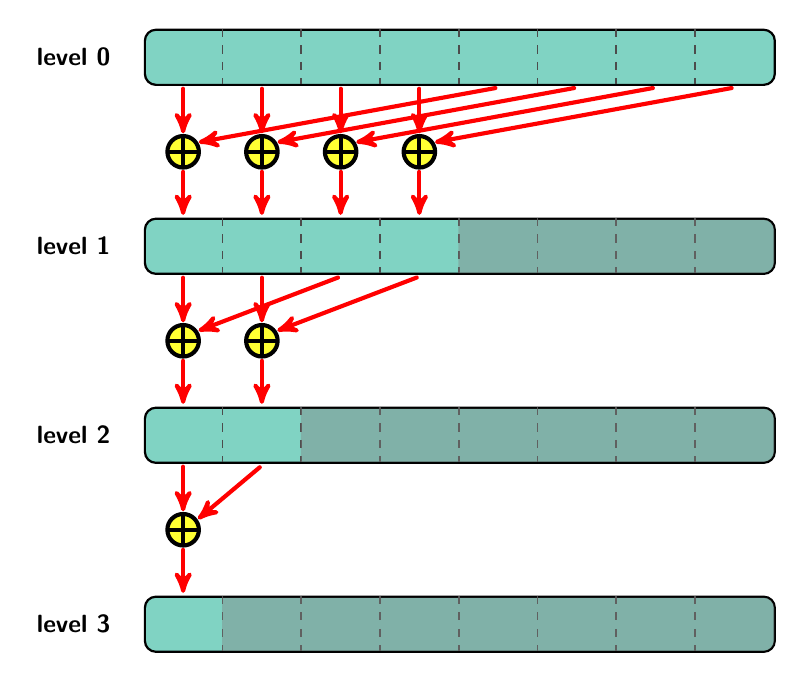
\begin{tikzpicture}[scale=1.0,transform shape]

  % Parameters
  \def\xcell{1.0cm}
  \def\ycell{0.7cm}
  \def\dtab{2.4cm}
  \def\radius{0.2cm}

  % Styles
  \tikzstyle{table}=[draw,anchor=north west,thick,rounded corners]
  \tikzstyle{line}=[dashed,line width=0.7pt]
  \tikzstyle{to}=[->,>=stealth',shorten <=1pt,shorten >=1pt,line width=1.5pt,red,cap=round]

  % \table*{<id>}{<pos>}{<x-dim>}{<y-dim>}{<cell-lalbel-list>}[<optional-arguments>]
  % The star (*) argument enables drawing of lines between the cells
  \DeclareDocumentCommand \table { s m m m m m O{} }{%
    \path #3 node[table,minimum width=#4*\xcell,minimum height=#5*\ycell,#7] (table-#2) {};
    \IfBooleanT{#1}{%
      \pgfmathsetmacro\xdim{#4-1}
      \pgfmathsetmacro\ydim{#5-1}
      \ifnumgreater{#5}{1}{%
        \foreach \y in {1,...,\ydim}
          \draw[line,Black!70] ($(table-#2.north west)+(0,-\y*\ycell)$) -- ++(#4*\xcell,0);}{}
      \ifnumgreater{#4}{1}{%
        \foreach \x in {1,...,\xdim}
          \draw[line,Black!70] ($(table-#2.north west)+(\x*\xcell,0)$) -- ++(0,-#5*\ycell);}{}
    }
    \foreach[count=\li from 0] \l in {#6}{%
      \pgfmathsetmacro\lx{mod(\li,#4) + 0.5}
      \pgfmathsetmacro\ly{int(\li/#4) + 0.5}
      \node (cell-label-#2-\li) at ($(table-#2.north west)+(\lx*\xcell,-\ly*\ycell)$) {\l};
    }
  }

  % \shade{<id>}{<num-cells>}{<pos>}
  \DeclareDocumentCommand \shade { m m m }{%
    \path ($#3+(-0.02,0)$) node[anchor=east,minimum width=#2*\xcell,minimum height=0.95*\ycell,append after command={\pgfextra \draw[draw=none,sharp corners,fill=gray,opacity=0.4] (\tikzlastnode.north) [rounded corners=4pt] -| (\tikzlastnode.east) [rounded corners=4pt] |- (\tikzlastnode.south) [rounded corners=0pt] -| (\tikzlastnode.west) [rounded corners=0pt] |- (\tikzlastnode.north); \endpgfextra}] (shade-#1) {};
  }

  % \adder{<top-table-id>}{<bottom-table-id>}{<op-cell-diff>}{<x-offset>}
  \DeclareDocumentCommand \adder { m m m m }{%
    \node[draw=none] (mid-dist) at ($(table-#1.south west)!0.5!(table-#2.north west)+(#4,0)$) {};
    \draw[line width=1.5pt,fill=Yellow!80] (mid-dist) circle (\radius);
    \draw[line width=1.5pt] ($(mid-dist)+(180:\radius)$) -- ($(mid-dist)+(0:\radius)$);
    \draw[line width=1.5pt] ($(mid-dist)+(-90:\radius)$) -- ($(mid-dist)+(90:\radius)$);
    \draw[to] ($(table-#1.south west)+(#4,0)$) -- ($(mid-dist)+(0,\radius)$);
    \draw[to] ($(mid-dist)+(0,{-\radius-0.02cm})$) -- (mid-dist |- table-#2.north);
    \draw[to] ($(table-#1.south west)+({#4+#3*\xcell},-0.02)$) -- ($(mid-dist)+(35:\radius)$);
  }

  % ===========================================================================
 
  % Draw level 0
  \table*{0}{(0,0)}{8}{1}{}[fill=Emerald!50]
  
  % Draw level 1
  \table*{1}{(0,-\dtab)}{8}{1}{}[fill=Emerald!50]
  \shade{1}{4}{(table-1.east)}
  \foreach \i in {0,1,2,3}{%
    \pgfmathsetmacro\offset{\i + 0.5}
    \adder{0}{1}{4}{\offset*\xcell}
  }

  % Draw level 2
  \table*{2}{(0,-2*\dtab)}{8}{1}{}[fill=Emerald!50]
  \shade{2}{6}{(table-2.east)}
  \foreach \i in {0,1}{%
    \pgfmathsetmacro\offset{\i + 0.5}
    \adder{1}{2}{2}{\offset*\xcell}
  }

  % Draw level 3
  \table*{3}{(0,-3*\dtab)}{8}{1}{}[fill=Emerald!50]
  \shade{3}{7}{(table-3.east)}
  \adder{2}{3}{1}{0.5*\xcell}

  % Draw labels
  \node[anchor=east] at ($(table-0.west)+(-0.3,0.0)$) {\sffamily\bfseries\small{level 0}};
  \node[anchor=east] at ($(table-1.west)+(-0.3,0.0)$) {\sffamily\bfseries\small{level 1}};
  \node[anchor=east] at ($(table-2.west)+(-0.3,0.0)$) {\sffamily\bfseries\small{level 2}};
  \node[anchor=east] at ($(table-3.west)+(-0.3,0.0)$) {\sffamily\bfseries\small{level 3}};

\end{tikzpicture}
\caption{Representation of reduce.}
\label{fig:reduce-parallel}
\end{figure}

\clearpage
%!TEX root = ../main.tex

\begin{figure}[p]
\centering
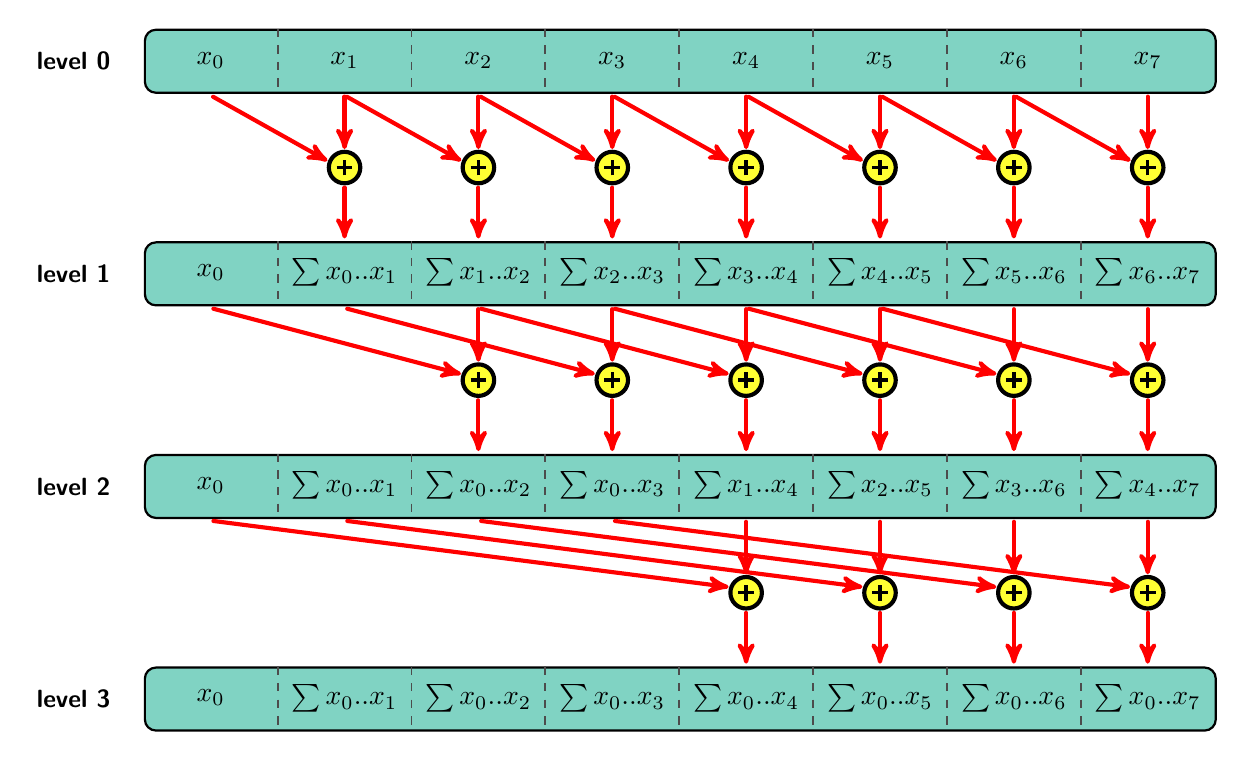
\begin{tikzpicture}[scale=1.0,transform shape]

  % Parameters
  \def\xcell{1.7cm}
  \def\ycell{0.8cm}
  \def\dtab{2.7cm}
  \def\radius{0.2cm}

  % Styles
  \tikzstyle{table}=[draw,anchor=north west,thick,rounded corners]
  \tikzstyle{line}=[dashed,line width=0.7pt]
  \tikzstyle{to}=[->,>=stealth',shorten <=1pt,shorten >=1pt,line width=1.5pt,red,cap=round]

  % \table*{<id>}{<pos>}{<x-dim>}{<y-dim>}{<cell-lalbel-list>}[<optional-arguments>]
  % The star (*) argument enables drawing of lines between the cells
  \DeclareDocumentCommand \table { s m m m m m O{} }{%
    \path #3 node[table,minimum width=#4*\xcell,minimum height=#5*\ycell,#7] (table-#2) {};
    \IfBooleanT{#1}{%
      \pgfmathsetmacro\xdim{#4-1}
      \pgfmathsetmacro\ydim{#5-1}
      \ifnumgreater{#5}{1}{%
        \foreach \y in {1,...,\ydim}
          \draw[line,Black!70] ($(table-#2.north west)+(0,-\y*\ycell)$) -- ++(#4*\xcell,0);}{}
      \ifnumgreater{#4}{1}{%
        \foreach \x in {1,...,\xdim}
          \draw[line,Black!70] ($(table-#2.north west)+(\x*\xcell,0)$) -- ++(0,-#5*\ycell);}{}
    }
    \foreach[count=\li from 0] \l in {#6}{%
      \pgfmathsetmacro\lx{mod(\li,#4) + 0.5}
      \pgfmathsetmacro\ly{int(\li/#4) + 0.5}
      \node (cell-label-#2-\li) at ($(table-#2.north west)+(\lx*\xcell,-\ly*\ycell)$) {\l};
    }
  }

  % \adder{<top-table-id>}{<bottom-table-id>}{<main-cell>}{<secondary-cell>}
  \DeclareDocumentCommand \adder { m m m m }{%
    \node (mid-dist) at ($(table-#1.south west)!0.5!(table-#2.north west)+(0.5*\xcell+#3*\xcell,0)$) {};
    \draw[line width=1.5pt,fill=Yellow!80] (mid-dist) circle (\radius);
    \draw[line width=1.2pt] ($(mid-dist)+(180:\radius-1mm)$) -- ($(mid-dist)+(0:\radius-1mm)$);
    \draw[line width=1.2pt] ($(mid-dist)+(-90:\radius-1mm)$) -- ($(mid-dist)+(90:\radius-1mm)$);
    \draw[to] (table-#1.south -| mid-dist) -- ($(mid-dist)+(0,\radius)$);
    \draw[to] ($(mid-dist)+(0,{-\radius-0.02cm})$) -- (mid-dist |- table-#2.north);
    \draw[to] ($(table-#1.south west)+({0.5*\xcell+#4*\xcell},-0.02)$) -- ($(mid-dist)+(160:\radius)$);
  }

  % ===========================================================================

  % Draw level 0
  \table*{0}{(0,0)}{8}{1}{$x_0$,$x_1$,$x_2$,$x_3$,$x_4$,$x_5$,$x_6$,$x_7$}[fill=Emerald!50]
  
  % Draw level 1
  \table*{1}{(0,-\dtab)}{8}{1}{$x_0$,$\sum x_0 .. x_1$,$\sum x_1 .. x_2$,$\sum x_2 .. x_3$,$\sum x_3 .. x_4$,$\sum x_4 .. x_5$,$\sum x_5 .. x_6$,$\sum x_6 .. x_7$}[fill=Emerald!50]
  \foreach[count=\j from 0] \i in {1,2,...,7}
    \adder{0}{1}{\i}{\j};

  % Draw level 2
  \table*{2}{(0,-2*\dtab)}{8}{1}{$x_0$,$\sum x_0 .. x_1$,$\sum x_0 .. x_2$,$\sum x_0 .. x_3$,$\sum x_1 .. x_4$,$\sum x_2 .. x_5$,$\sum x_3 .. x_6$,$\sum x_4 .. x_7$}[fill=Emerald!50]
  \foreach[count=\j from 0] \i in {2,3,...,7}
    \adder{1}{2}{\i}{\j};

  % Draw level 3
  \table*{3}{(0,-3*\dtab)}{8}{1}{$x_0$,$\sum x_0 .. x_1$,$\sum x_0 .. x_2$,$\sum x_0 .. x_3$,$\sum x_0 .. x_4$,$\sum x_0 .. x_5$,$\sum x_0 .. x_6$,$\sum x_0 .. x_7$}[fill=Emerald!50]
  \foreach[count=\j from 0] \i in {4,5,...,7}
    \adder{2}{3}{\i}{\j};

  % Draw labels
  \node[anchor=east] at ($(table-0.west)+(-0.3,0.0)$) {\sffamily\bfseries\small{level 0}};
  \node[anchor=east] at ($(table-1.west)+(-0.3,0.0)$) {\sffamily\bfseries\small{level 1}};
  \node[anchor=east] at ($(table-2.west)+(-0.3,0.0)$) {\sffamily\bfseries\small{level 2}};
  \node[anchor=east] at ($(table-3.west)+(-0.3,0.0)$) {\sffamily\bfseries\small{level 3}};

\end{tikzpicture}
\caption{Representation of Hillis \& Steele (sum) scan.}
\label{fig:hillis-scan}
\end{figure}

\clearpage
%!TEX root = ../main.tex

\begin{figure}[p]
\centering
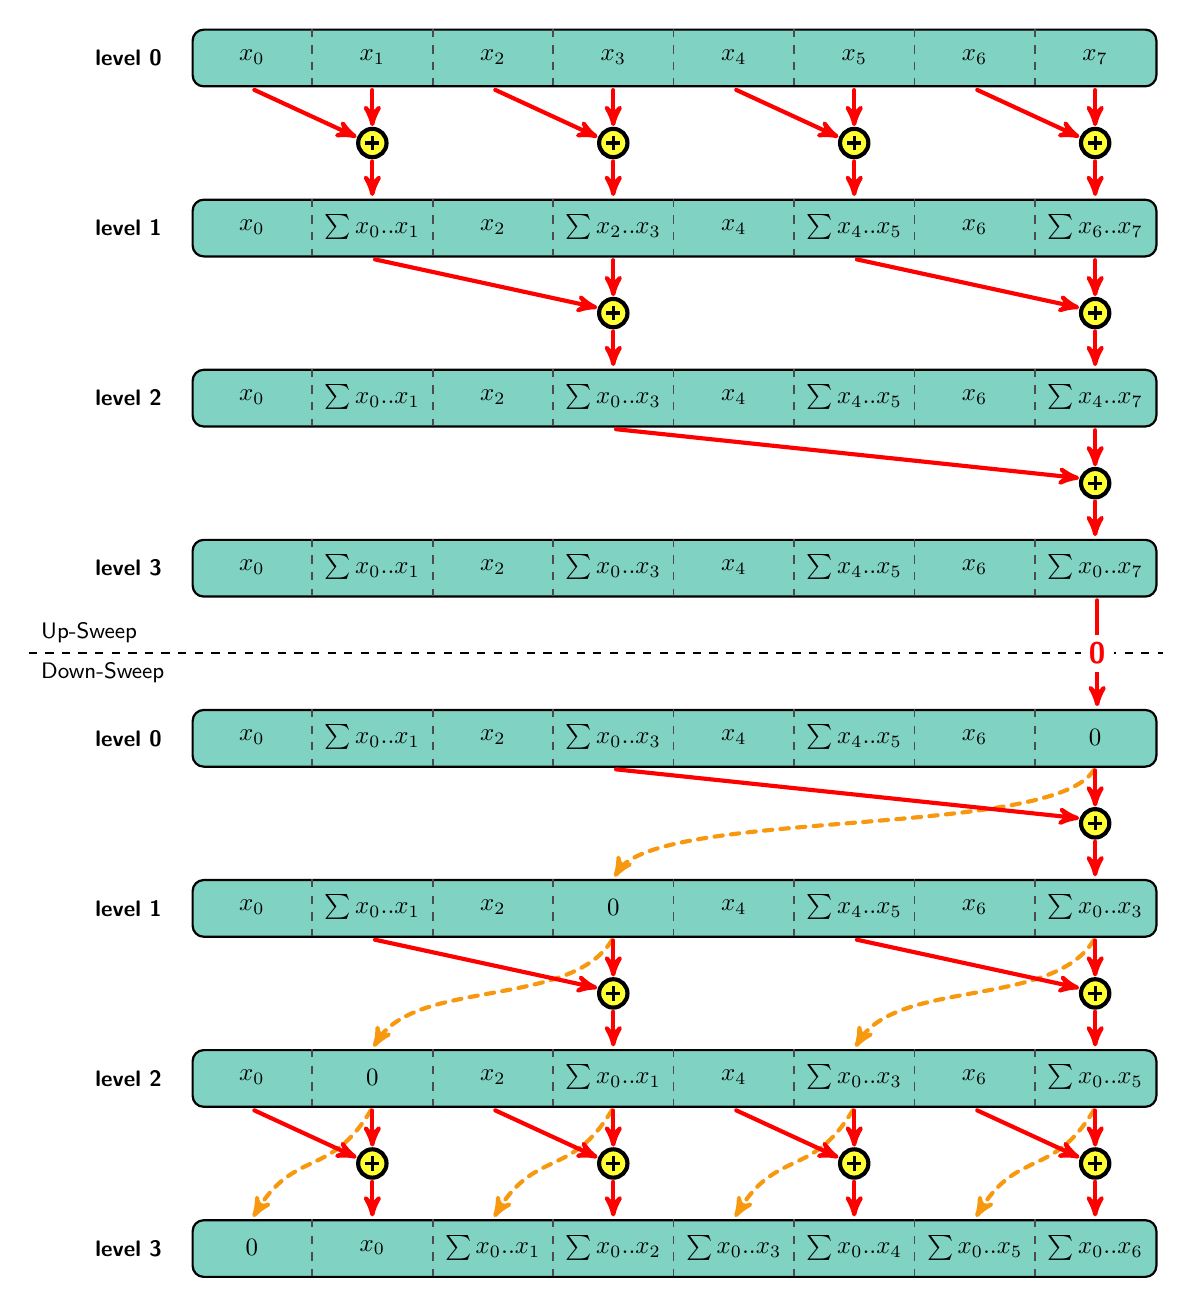
\begin{tikzpicture}[scale=0.9,transform shape]

  % Parameters
  \def\xcell{1.7cm}
  \def\ycell{0.8cm}
  \def\dtab{2.4cm}
  \def\radius{0.2cm}

  % Styles
  \tikzstyle{table}=[draw,anchor=north west,thick,rounded corners]
  \tikzstyle{line}=[dashed,line width=0.7pt]
  \tikzstyle{to}=[->,>=stealth',shorten <=1pt,shorten >=1pt,line width=1.5pt,red,cap=round]

  % \table*{<id>}{<pos>}{<x-dim>}{<y-dim>}{<cell-lalbel-list>}[<optional-arguments>]
  % The star (*) argument enables drawing of lines between the cells
  \DeclareDocumentCommand \table { s m m m m m O{} }{%
    \path #3 node[table,minimum width=#4*\xcell,minimum height=#5*\ycell,#7] (table-#2) {};
    \IfBooleanT{#1}{%
      \pgfmathsetmacro\xdim{#4-1}
      \pgfmathsetmacro\ydim{#5-1}
      \ifnumgreater{#5}{1}{%
        \foreach \y in {1,...,\ydim}
          \draw[line,Black!70] ($(table-#2.north west)+(0,-\y*\ycell)$) -- ++(#4*\xcell,0);}{}
      \ifnumgreater{#4}{1}{%
        \foreach \x in {1,...,\xdim}
          \draw[line,Black!70] ($(table-#2.north west)+(\x*\xcell,0)$) -- ++(0,-#5*\ycell);}{}
    }
    \foreach[count=\li from 0] \l in {#6}{%
      \pgfmathsetmacro\lx{mod(\li,#4) + 0.5}
      \pgfmathsetmacro\ly{int(\li/#4) + 0.5}
      \node (cell-label-#2-\li) at ($(table-#2.north west)+(\lx*\xcell,-\ly*\ycell)$) {\l};
    }
  }

  % \adderup{<top-table-id>}{<bottom-table-id>}{<main-cell>}{<secondary-cell>}
  \DeclareDocumentCommand \adderup { m m m m }{%
    \node (mid-dist) at ($(table-#1.south west)!0.5!(table-#2.north west)+(0.5*\xcell+#3*\xcell,0)$) {};
    \draw[line width=1.5pt,fill=Yellow!80] (mid-dist) circle (\radius);
    \draw[line width=1.2pt] ($(mid-dist)+(180:\radius-1mm)$) -- ($(mid-dist)+(0:\radius-1mm)$);
    \draw[line width=1.2pt] ($(mid-dist)+(-90:\radius-1mm)$) -- ($(mid-dist)+(90:\radius-1mm)$);
    \draw[to] (table-#1.south -| mid-dist) -- ($(mid-dist)+(0,\radius)$);
    \draw[to] ($(mid-dist)+(0,{-\radius-0.02cm})$) -- (mid-dist |- table-#2.north);
    \draw[to] ($(table-#1.south west)+({0.5*\xcell+#4*\xcell},-0.02)$) -- ($(mid-dist)+(160:\radius)$);
  }

  % \adderdown{<top-table-id>}{<bottom-table-id>}{<main-cell>}{<secondary-cell>}
  \DeclareDocumentCommand \adderdown { m m m m }{%
    \draw[to,dashed,YellowOrange] ($(table-#1.south west)+(0.5*\xcell+#3*\xcell,0)$) .. controls ++(-0.6,-1) and ++(0.6,1) .. ($(table-#2.north west)+({0.5*\xcell+#4*\xcell},0)$);
    \adderup{#1}{#2}{#3}{#4}
  }

  % ===========================================================================
 
  % Up-sweep
  \table*{0}{(0,0)}{8}{1}{$x_0$,$x_1$,$x_2$,$x_3$,$x_4$,$x_5$,$x_6$,$x_7$}[fill=Emerald!50]
  \table*{1}{(0,-\dtab)}{8}{1}{$x_0$,$\sum x_0 .. x_1$,$x_2$,$\sum x_2 .. x_3$,$x_4$,$\sum x_4 .. x_5$,$x_6$,$\sum x_6 .. x_7$}[fill=Emerald!50]
  \table*{2}{(0,-2*\dtab)}{8}{1}{$x_0$,$\sum x_0 .. x_1$,$x_2$,$\sum x_0 .. x_3$,$x_4$,$\sum x_4 .. x_5$,$x_6$,$\sum x_4 .. x_7$}[fill=Emerald!50]
  \table*{3}{(0,-3*\dtab)}{8}{1}{$x_0$,$\sum x_0 .. x_1$,$x_2$,$\sum x_0 .. x_3$,$x_4$,$\sum x_4 .. x_5$,$x_6$,$\sum x_0 .. x_7$}[fill=Emerald!50]
  
  \adderup{0}{1}{1}{0}
  \adderup{0}{1}{3}{2}
  \adderup{0}{1}{5}{4}
  \adderup{0}{1}{7}{6}

  \adderup{1}{2}{3}{1}
  \adderup{1}{2}{7}{5}

  \adderup{2}{3}{7}{3}

  % Down-sweep
  \table*{4}{(0,-4*\dtab)}{8}{1}{$x_0$,$\sum x_0 .. x_1$,$x_2$,$\sum x_0 .. x_3$,$x_4$,$\sum x_4 .. x_5$,$x_6$,$0$}[fill=Emerald!50]
  \table*{5}{(0,-5*\dtab)}{8}{1}{$x_0$,$\sum x_0 .. x_1$,$x_2$,$0$,$x_4$,$\sum x_4 .. x_5$,$x_6$,$\sum x_0 .. x_3$}[fill=Emerald!50]
  \table*{6}{(0,-6*\dtab)}{8}{1}{$x_0$,$0$,$x_2$,$\sum x_0 .. x_1$,$x_4$,$\sum x_0 .. x_3$,$x_6$,$\sum x_0 .. x_5$}[fill=Emerald!50]
  \table*{7}{(0,-7*\dtab)}{8}{1}{$0$,$x_0$,$\sum x_0 .. x_1$,$\sum x_0 .. x_2$,$\sum x_0 .. x_3$,$\sum x_0 .. x_4$,$\sum x_0 .. x_5$,$\sum x_0 .. x_6$}[fill=Emerald!50]

  \adderdown{4}{5}{7}{3}

  \adderdown{5}{6}{3}{1}
  \adderdown{5}{6}{7}{5}

  \adderdown{6}{7}{1}{0}
  \adderdown{6}{7}{3}{2}
  \adderdown{6}{7}{5}{4}
  \adderdown{6}{7}{7}{6}

  % Separator
  \draw[line] ($(table-3.west)+(-2.3,-0.5*\dtab)$) -- node[pos=0.003,anchor=west,yshift=8pt] {\sffamily\small Up-Sweep} node[pos=0.003,anchor=west,yshift=-8pt] {\sffamily\small Down-Sweep} ++(16,0);
  \draw[to] ($(table-3.south east)+(-0.5*\xcell,0)$) -- node[fill=white] {\sffamily\bfseries\large 0} ($(table-4.north east)+(-0.5*\xcell,0)$);

  % Labels
  \foreach \id/\l in {0/0,1/1,2/2,3/3,4/0,5/1,6/2,7/3}
    \node[anchor=east] at ($(table-\id.west)+(-0.3,0.0)$) {\sffamily\bfseries\small{level \l}};

\end{tikzpicture}
\caption{Representation of Blelloch (sum) scan.}
\label{fig:blelloch-scan}
\end{figure}

\clearpage
%!TEX root = ../main.tex

\begin{figure}[p]
\centering
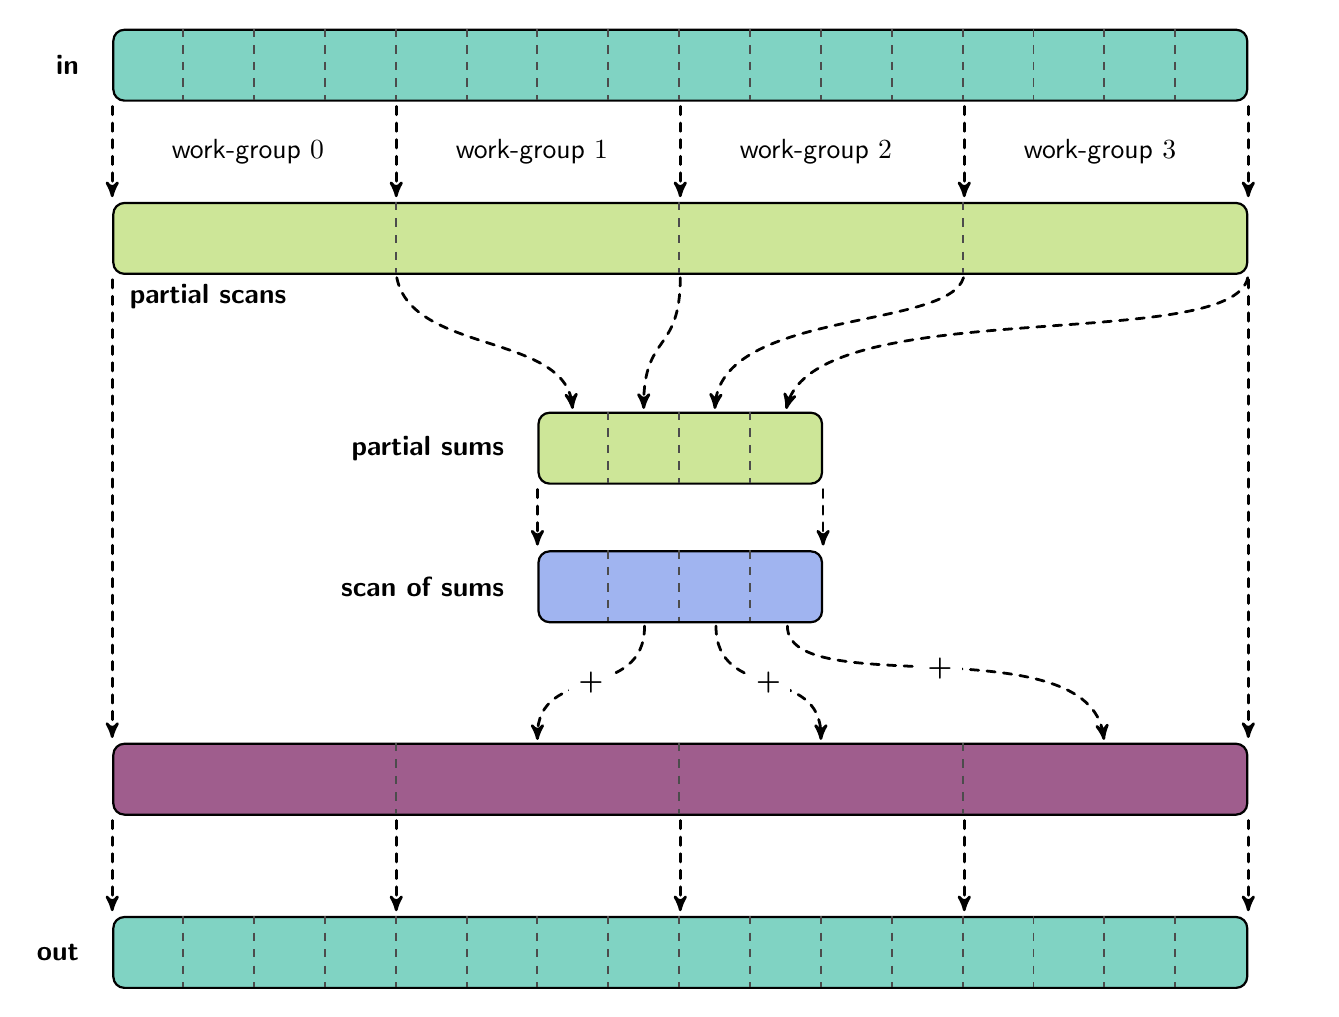
\begin{tikzpicture}[scale=1.0,transform shape]

  % Parameters
  \def\xcell{0.9cm}
  \def\ycell{0.9cm}
  \def\dtab{2.2cm}

  % Styles
  \tikzstyle{table}=[draw,anchor=north west,thick,rounded corners]
  \tikzstyle{line}=[dashed,line width=0.7pt]
  \tikzstyle{to}=[->,>=stealth',shorten <=1pt,shorten >=1pt,line width=1.5pt,red,cap=round]
  \tikzstyle{bline}=[to,dashed,line width=1.0pt,black]

  % \table*{<id>}{<pos>}{<x-dim>}{<y-dim>}{<cell-lalbel-list>}[<optional-arguments>]
  % The star (*) argument enables drawing of lines between the cells
  \DeclareDocumentCommand \table { s m m m m m O{} }{%
    \path #3 node[table,minimum width=#4*\xcell,minimum height=#5*\ycell,#7] (table-#2) {};
    \IfBooleanT{#1}{%
      \pgfmathsetmacro\xdim{#4-1}
      \pgfmathsetmacro\ydim{#5-1}
      \ifnumgreater{#5}{1}{%
        \foreach \y in {1,...,\ydim}
          \draw[line,Black!70] ($(table-#2.north west)+(0,-\y*\ycell)$) -- ++(#4*\xcell,0);}{}
      \ifnumgreater{#4}{1}{%
        \foreach \x in {1,...,\xdim}
          \draw[line,Black!70] ($(table-#2.north west)+(\x*\xcell,0)$) -- ++(0,-#5*\ycell);}{}
    }
    \foreach[count=\li from 0] \l in {#6}{%
      \pgfmathsetmacro\lx{mod(\li,#4) + 0.5}
      \pgfmathsetmacro\ly{int(\li/#4) + 0.5}
      \node (cell-label-#2-\li) at ($(table-#2.north west)+(\lx*\xcell,-\ly*\ycell)$) {\l};
    }
  }

  % \bline{<top-table-id>}{<bottom-table-id>}{<num-lines> - 1}{<label-list>}[<x-shift>]
  \DeclareDocumentCommand \bline { m m m m O{0pt} }{%
    \pgfmathsetmacro\xrel{1/#3}
    \foreach[count=\li from 0] \l in {#4}{%
      \node[inner sep=0pt] (top) at ($(table-#1.south west)!{\li*\xrel}!(table-#1.south east)$) {};
      \node[inner sep=0pt] (bottom) at ($(table-#2.north west)!{\li*\xrel}!(table-#2.north east)$) {};
      \draw[bline] (top) -- (bottom);
      \node[anchor=west,inner sep=0pt,xshift=#5] at ($(top)!0.5!(bottom)$) {\sffamily \l};
    }
  }

  % ===========================================================================
 
  % Work-group scans
  \table*{0}{(0,0)}{16}{1}{}[fill=Emerald!50]
  \def\xcell{4*0.9cm}
  \table*{1}{(0,-\dtab)}{4}{1}{}[fill=YellowGreen!50]
  \def\xcell{0.9cm}
  \bline{0}{1}{4}{work-group $0$,work-group $1$,work-group $2$,work-group $3$,}[7.5mm]

  % Work-group sums
  \table*{2}{($(table-1)+(0,-\dtab)$)}{4}{1}{}[anchor=north,fill=YellowGreen!50]
  \draw[bline] ($(table-1.south west)!0.25!(table-1.south east)$) .. controls ++(0.2,-1) and ++(-0.1,1) .. ($(table-2.north west)+(0.5*\xcell,0)$);
  \draw[bline] ($(table-1.south west)!0.5!(table-1.south east)$) .. controls ++(0,-1) and ++(0,1) .. ($(table-2.north west)+(1.5*\xcell,0)$);
  \draw[bline] ($(table-1.south west)!0.75!(table-1.south east)$) .. controls ++(-0.2,-0.7) and ++(0.1,1.3) .. ($(table-2.north west)+(2.5*\xcell,0)$);
  \draw[bline] ($(table-1.south west)!1.0!(table-1.south east)$) .. controls ++(-0.2,-1) and ++(0.4,1.5) .. ($(table-2.north west)+(3.5*\xcell,0)$);

  % Sums scan
  \table*{3}{($(table-2.south)+(0,-0.8*\dtab)$)}{4}{1}{}[anchor=south,fill=RoyalBlue!50]
  \bline{2}{3}{1}{,}

  % Sums addition
  \def\xcell{4*0.9cm}
  \table*{4}{($(table-1.south west)+(0,-2.7*\dtab)$)}{4}{1}{}[fill=RoyalBlue!50!YellowGreen!50!VioletRed]
  \def\xcell{0.9cm}
  \table*{5}{($(table-4.north west)+(0,-\dtab)$)}{16}{1}{}[fill=Emerald!50]
  \bline{1}{4}{1}{,}
  \bline{4}{5}{4}{,,,,}

  % Global sums lines
  \draw[bline] ($(table-3.south west)!{3*0.125}!(table-3.south east)$) .. controls ++(0,-1) and ++(0,1) .. node[fill=white] {$\bm +$} ($(table-4.north west)+(1.5*4*\xcell,0)$);
  \draw[bline] ($(table-3.south west)!{5*0.125}!(table-3.south east)$) .. controls ++(0,-1) and ++(0,1) .. node[fill=white] {$\bm +$} ($(table-4.north west)+(2.5*4*\xcell,0)$);
  \draw[bline] ($(table-3.south west)!{7*0.125}!(table-3.south east)$) .. controls ++(-0,-1) and ++(-0.2,1.5) .. node[fill=white] {$\bm +$} ($(table-4.north west)+(3.5*4*\xcell,0)$);

  % Labels
  \node[anchor=east] at ($(table-0.west)+(-0.3,0)$) {\sffamily\bfseries{in}};
  \node[anchor=north west] at ($(table-1.south west)+(0.1,0)$) {\sffamily\bfseries{partial scans}};
  \node[anchor=east] at ($(table-2.west)+(-0.3,0)$) {\sffamily\bfseries{partial sums}};
  \node[anchor=east] at ($(table-3.west)+(-0.3,0)$) {\sffamily\bfseries{scan of sums}};
  \node[anchor=east] at ($(table-5.west)+(-0.3,0)$) {\sffamily\bfseries{out}};

\end{tikzpicture}
\caption{Representation of Blelloch (sum) scan for arbitrary size input.}
\label{fig:blelloch-scan-sums}
\end{figure}

\clearpage
%!TEX root = ../main.tex

\begin{figure}[p]
\centering
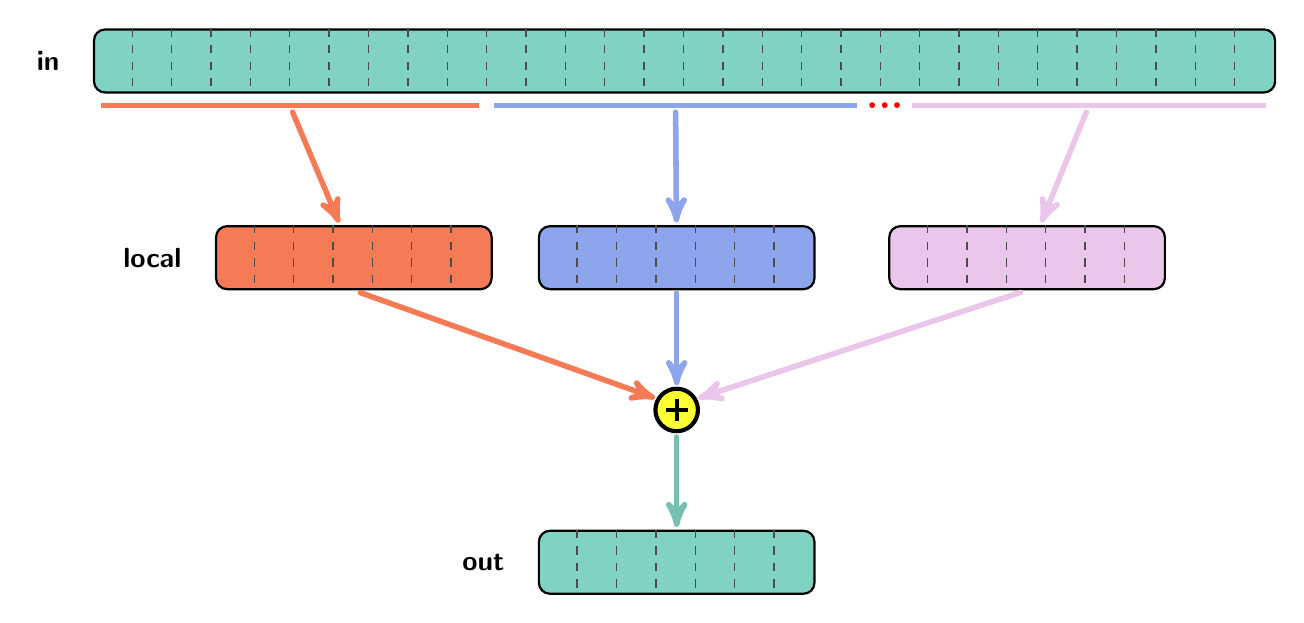
\begin{tikzpicture}[scale=1.0,transform shape]

  \def\xcell{0.5cm}
  \def\ycell{0.8cm}
  \def\dist{1.9*\ycell}
  \def\radius{2.7mm}

  % Styles
  \tikzstyle{table}=[draw,anchor=north west,thick,rounded corners]
  \tikzstyle{line}=[dashed,line width=0.5pt]
  \tikzstyle{to}=[->,>=stealth',shorten <=1pt,shorten >=1pt,line width=2pt,red,cap=round]

  % \table*{<id>}{<pos>}{<x-dim>}{<y-dim>}{<cell-lalbel-list>}[<optional-arguments>]
  % The star (*) argument enables drawing of lines between the cells
  \DeclareDocumentCommand \table { s m m m m m O{} }{%
    \path #3 node[table,minimum width=#4*\xcell,minimum height=#5*\ycell,#7] (table-#2) {};
    \IfBooleanT{#1}{%
      \pgfmathsetmacro\xdim{#4-1}
      \pgfmathsetmacro\ydim{#5-1}
      \ifnumgreater{#5}{1}{%
        \foreach \y in {1,...,\ydim}
          \draw[line,Black!70] ($(table-#2.north west)+(0,-\y*\ycell)$) -- ++(#4*\xcell,0);}{}
      \ifnumgreater{#4}{1}{%
        \foreach \x in {1,...,\xdim}
          \draw[line,Black!70] ($(table-#2.north west)+(\x*\xcell,0)$) -- ++(0,-#5*\ycell);}{}
    }
    \foreach[count=\li from 0] \l in {#6}{%
      \pgfmathsetmacro\lx{mod(\li,#4) + 0.5}
      \pgfmathsetmacro\ly{int(\li/#4) + 0.5}
      \node (cell-label-#2-\li) at ($(table-#2.north west)+(\lx*\xcell,-\ly*\ycell)$) {\l};
    }
  }

  % ===========================================================================

  % Draw input
  \table*{0}{(0,0)}{30}{1}{}[fill=Emerald!50]

  % Draw group declarative lines
  \draw[inner sep=0pt,line width=2pt,RedOrange!70] ($(table-0.south west)+(1mm,-1.5mm)$) -- node[midway] (line-0) {} ++($(10*\xcell,0)+(-2mm,0)$);
  \draw[inner sep=0pt,line width=2pt,RoyalBlue!60] ($(table-0.south west)+(1mm+10*\xcell,-1.5mm)$) -- node[midway] (line-1) {} ++($(10*\xcell,0)+(-4mm,0)$);
  \draw[inner sep=0pt,line width=2pt,Plum!60] ($(table-0.south west)+(4mm+20*\xcell,-1.5mm)$) -- node[midway] (line-2) {} ++($(10*\xcell,0)+(-5mm,0)$);
  \node[Red] at ($(line-1)!0.506!(line-2)$) {\Large\bfseries...};

  % Draw local histograms
  \table*{1}{($(line-0)+(-1.5*\xcell-2mm,-\dist)$)}{7}{1}{}[fill=RedOrange!70]
  \table*{2}{($(line-1)+(-3.5*\xcell,-\dist)$)}{7}{1}{}[fill=RoyalBlue!60]
  \table*{3}{($(line-2)+(-5.5*\xcell+2mm,-\dist)$)}{7}{1}{}[fill=Plum!60]
  \draw[to,RedOrange!70] (line-0) -- (table-1);
  \draw[to,RoyalBlue!60] (line-1) -- (table-2);
  \draw[to,Plum!60] (line-2) -- (table-3);

  % Draw output
  \table*{4}{($(table-2.south)+(0,-2*\dist)$)}{7}{1}{}[fill=Emerald!50,anchor=north]
  
  % Draw adder
  \node (mid-dist) at ($(table-2.south)+(0,-\dist)$) {};
  \draw[line width=1.5pt,fill=Yellow!80] (mid-dist) circle (\radius);
  \draw[line width=1.5pt] ($(mid-dist)+(180:\radius-1.3mm)$) -- ($(mid-dist)+(0:\radius-1.3mm)$);
  \draw[line width=1.5pt] ($(mid-dist)+(-90:\radius-1.3mm)$) -- ($(mid-dist)+(90:\radius-1.3mm)$);
  \draw[to,shorten <=2.5pt,RedOrange!70] (table-1.south) -- ($(mid-dist)+(150:\radius+0.1mm)$);
  \draw[to,RoyalBlue!60] (table-2.south) -- ($(mid-dist)+(90:\radius+0.1mm)$);
  \draw[to,shorten <=2.5pt,Plum!60] (table-3.south) -- ($(mid-dist)+(30:\radius+0.1mm)$);
  \draw[to,Emerald!70!Gray!70!White] ($(mid-dist)+(-90:\radius+0.4mm)$) -- (table-4.north);

  % Draw labels
  \node[draw=none,anchor=east] at ($(table-0.west)+(-0.3,0.0)$) {\sffamily\bfseries{in}};
  \node[draw=none,anchor=east] at ($(table-1.west)+(-0.3,0.0)$) {\sffamily\bfseries{local}};
  \node[draw=none,anchor=east] at ($(table-4.west)+(-0.3,0.0)$) {\sffamily\bfseries{out}};

\end{tikzpicture}
\caption{Representation of histogram.}
\label{fig:histogram}
\end{figure}

\clearpage
%!TEX root = ../main.tex

\begin{figure}[p]
\centering
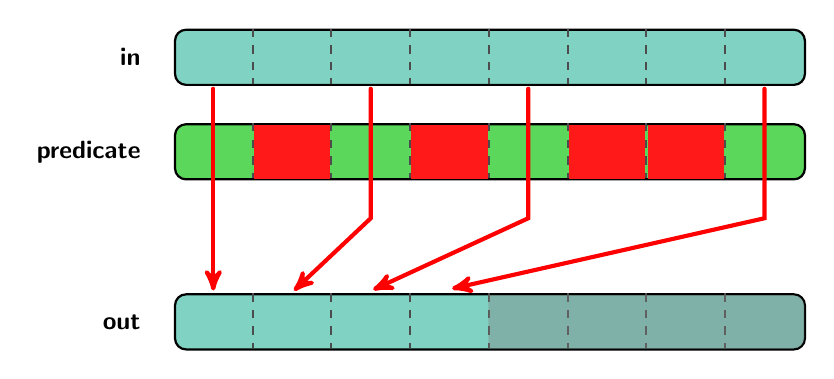
\begin{tikzpicture}[scale=1.0,transform shape]

  % Parameters
  \def\xcell{1.0cm}
  \def\ycell{0.7cm}
  \def\dtab{2.4cm}
  \def\radius{0.2cm}

  % Styles
  \tikzstyle{table}=[draw,anchor=north west,thick,rounded corners]
  \tikzstyle{cell}=[anchor=west,fill=red!90,text centered,minimum width=\xcell-0.03cm,minimum height=\ycell-0.02cm,inner sep=0.3cm]
  \tikzstyle{line}=[dashed,line width=0.7pt]
  \tikzstyle{to}=[->,>=stealth',shorten <=1pt,shorten >=1pt,line width=1.5pt,red,cap=round]

  % \table*{<id>}{<pos>}{<x-dim>}{<y-dim>}{<cell-lalbel-list>}[<optional-arguments>]
  % The star (*) argument enables drawing of lines between the cells
  \DeclareDocumentCommand \table { s m m m m m O{} }{%
    \path #3 node[table,minimum width=#4*\xcell,minimum height=#5*\ycell,#7] (table-#2) {};
    \IfBooleanT{#1}{%
      \pgfmathsetmacro\xdim{#4-1}
      \pgfmathsetmacro\ydim{#5-1}
      \ifnumgreater{#5}{1}{%
        \foreach \y in {1,...,\ydim}
          \draw[line,Black!70] ($(table-#2.north west)+(0,-\y*\ycell)$) -- ++(#4*\xcell,0);}{}
      \ifnumgreater{#4}{1}{%
        \foreach \x in {1,...,\xdim}
          \draw[line,Black!70] ($(table-#2.north west)+(\x*\xcell,0)$) -- ++(0,-#5*\ycell);}{}
    }
    \foreach[count=\li from 0] \l in {#6}{%
      \pgfmathsetmacro\lx{mod(\li,#4) + 0.5}
      \pgfmathsetmacro\ly{int(\li/#4) + 0.5}
      \node (cell-label-#2-\li) at ($(table-#2.north west)+(\lx*\xcell,-\ly*\ycell)$) {\l};
    }
  }

  % \shade{<id>}{<num-cells>}{<pos>}
  \DeclareDocumentCommand \shade { m m m }{%
    \path ($#3+(-0.02,0)$) node[anchor=east,minimum width=#2*\xcell,minimum height=0.95*\ycell,append after command={\pgfextra \draw[draw=none,sharp corners,fill=gray,opacity=0.4] (\tikzlastnode.north) [rounded corners=4pt] -| (\tikzlastnode.east) [rounded corners=4pt] |- (\tikzlastnode.south) [rounded corners=0pt] -| (\tikzlastnode.west) [rounded corners=0pt] |- (\tikzlastnode.north); \endpgfextra}] (shade-#1) {};
  }

  % \cell{<table-id>}{<cell-id>}
  \DeclareDocumentCommand \cell { m m }{%
    \path ($(table-#1.west)+({#2*\xcell+0.008cm},0)$) node[cell] {};
  }

  % \link{<top-table-id>}{<bottom-table-id>}{<top-table-cell>}{<top-table-cell>}[<arrow-tip-y-offset>]
  \DeclareDocumentCommand \link { m m m m O{0} }{%
    \draw[to] ($(table-#1.south west)+(#3*\xcell+0.5*\xcell,0)$) -- ++(0,-0.7*\dtab) -- ($(table-#2.north west)+(#4*\xcell+0.5*\xcell,#5)$);
  }

  % ===========================================================================

  % Draw input
  \table*{0}{(0,0)}{8}{1}{}[fill=Emerald!50]
  
  % Draw predicate
  \table*{1}{(0.0,-0.5*\dtab)}{8}{1}{}[fill=LimeGreen!80]
  \cell{1}{1}
  \cell{1}{3}
  \cell{1}{5}
  \cell{1}{6}

  % Draw output
  \table*{2}{(0.0,-1.4*\dtab)}{8}{1}{}[fill=Emerald!50]
  \shade{2}{4}{(table-2.east)}

  % Draw mapping lines
  \foreach \tc/\bc/\y in {0/0/0,2/1/0.01,4/2/0.03,7/3/0.05}
    \link{0}{2}{\tc}{\bc}[\y];

  % Draw labels
  \node[anchor=east] at ($(table-0.west)+(-0.3,0.0)$) {\sffamily\bfseries\small{in}};
  \node[anchor=east] at ($(table-1.west)+(-0.3,0.0)$) {\sffamily\bfseries\small{predicate}};
  \node[anchor=east] at ($(table-2.west)+(-0.3,0.0)$) {\sffamily\bfseries\small{out}};

\end{tikzpicture}
\caption{Representation of compact.}
\label{fig:compact}
\end{figure}

\clearpage
%!TEX root = ../main.tex

\begin{figure}[p]
\centering
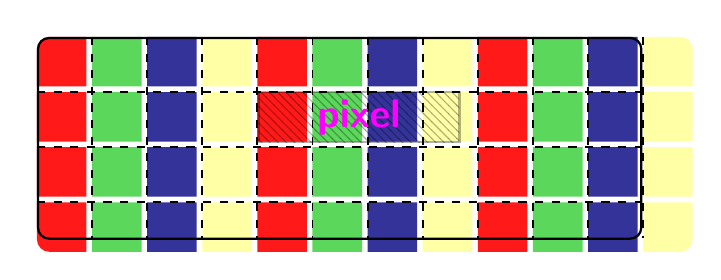
\begin{tikzpicture}[scale=1.0,transform shape]

  % Parameters
  \def\wtab{21.8em}
  \def\htab{7.25em}
  \def\celldim{0.7}

  % Styles
  \tikzstyle{table}=[draw,thick,rounded corners,text centered,minimum width=\wtab,minimum height=\htab,inner sep=0.3cm]
  \tikzstyle{cell}=[anchor=north west,text centered,minimum width=1.8em-0.05em,minimum height=1.8em-0.05em,inner sep=0.3cm]
  \tikzstyle{shade}=[draw,thick,anchor=north west,fill=gray,opacity=0.3,pattern=north west lines,text centered]
  \tikzstyle{sep}=[dashed,line width=0.7pt]

  % \frame{<id>}{<pos>}[<fill-color>]
  \DeclareDocumentCommand \frame { m m o }{%
    \path #2 node[table,anchor=north west,fill=\IfValueTF{#3}{#3}{none}] (frame-#1) {};
    \foreach \x in {1,2,...,11}
      \draw[sep] ($(frame-#1.north west)+(\x*\celldim,0)$) -- ++(0,-\htab);
    \foreach \y in {1,2,3}
      \draw[sep] ($(frame-#1.north west)+(0,-\y*\celldim)$) -- ++(\wtab,0);
  }

  % \cell{<pos>}{<cell-x-id>}{<cell-y-id>}{<color>}[<north-west-arc>][<south-west-arc>][<north-east-arc>][<south-east-arc>]
  \DeclareDocumentCommand \cell { m m m m O{0pt} O{0pt} O{0pt} O{0pt} }{%
    \path ($#1+({#2*\celldim},{-#3*\celldim})$) node[cell,append after command={\pgfextra \draw[draw=none,sharp corners,fill=#4] (\tikzlastnode.north) [rounded corners=#7] -| (\tikzlastnode.east) [rounded corners=#8] |- (\tikzlastnode.south) [rounded corners=#6] -| (\tikzlastnode.west) [rounded corners=#5] |- (\tikzlastnode.north); \endpgfextra}] {};
  }

  % \shade{<pos>}{<x-cells>}{<y-cells>}{<label>}
  \DeclareDocumentCommand \shade { m m m m }{%
    \path #1 node[shade,minimum width=#2*1.815em,minimum height=#3*1.8em] (shade) {};
    \node[text=Fuchsia] at (shade) {\sffamily\bfseries\Large #4};
  }

  % ===========================================================================

  % Create reference point
  \node (p) at (0,0) {};

  % Draw R channel
  \foreach \y in {1,2}
    \cell{(p)}{0}{\y}{Red!90};
  \cell{(p)}{0}{0}{Red!90}[4.5pt]
  \cell{(p)}{0}{3}{Red!90}[0pt][4.5pt]
  \foreach \x in {4,8}
    \foreach \y in {0,1,...,3}
      \cell{(p)}{\x}{\y}{Red!90};

  % Draw G channel
  \foreach \x in {1,5,9}
    \foreach \y in {0,1,...,3}
      \cell{(p)}{\x}{\y}{LimeGreen!80};

  % Draw B channel
  \foreach \x in {2,6,10}
    \foreach \y in {0,1,...,3}
      \cell{(p)}{\x}{\y}{NavyBlue!80};

  % Draw A channel
  \foreach \y in {1,2}
    \cell{(p)}{11}{\y}{Yellow!35};
  \cell{(p)}{11}{0}{Yellow!35}[0pt][0pt][4.5pt]
  \cell{(p)}{11}{3}{Yellow!35}[0pt][0pt][0pt][4.5pt]
  \foreach \x in {3,7}
    \foreach \y in {0,1,...,3}
      \cell{(p)}{\x}{\y}{Yellow!35};

  % Draw frame
  \frame{0}{(p)}

  % Draw shade
  \shade{($(frame-0.north west)+(4*\celldim,-\celldim+0.01)$)}{4}{1}{pixel}

\end{tikzpicture}
\caption{Representation of a $3 \times 4$ RGBA image.}
\label{fig:rgba}
\end{figure}

\clearpage
%!TEX root = ../main.tex

\begin{figure}[p]
\centering
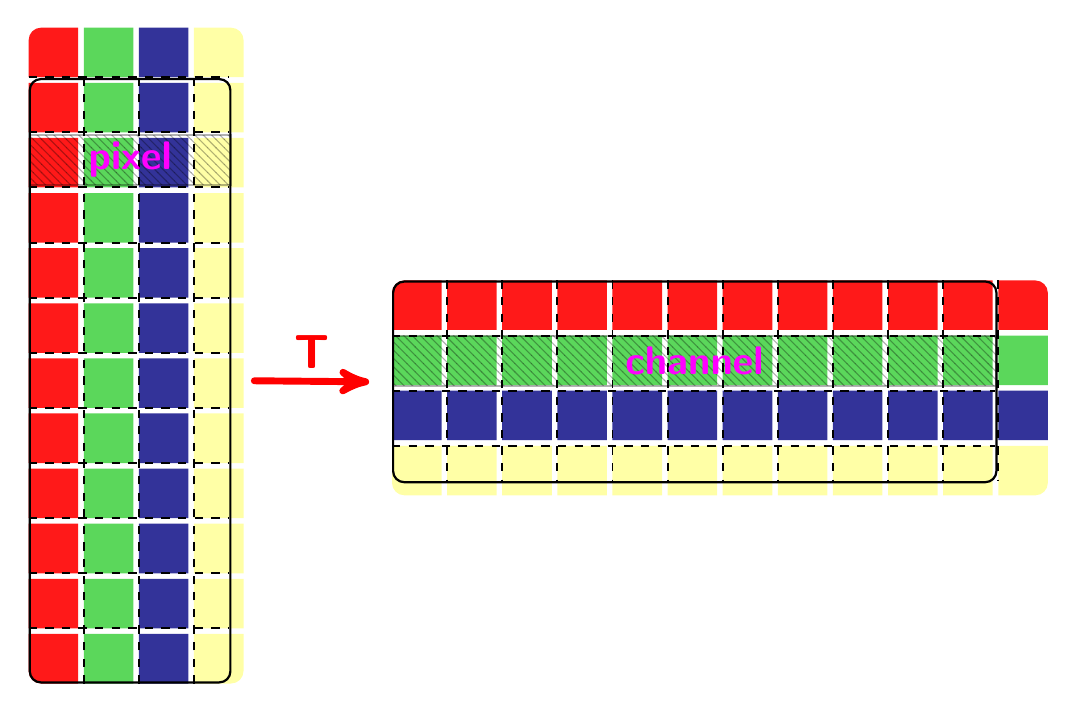
\begin{tikzpicture}[scale=1.0,transform shape]

  % Parameters
  \def\wtab{21.8em}
  \def\htab{7.25em}
  \def\celldim{0.7}

  % Styles
  \tikzstyle{table}=[draw,thick,rounded corners,text centered,minimum width=\wtab,minimum height=\htab,inner sep=0.3cm]
  \tikzstyle{cell}=[anchor=north west,text centered,minimum width=1.8em-0.05em,minimum height=1.8em-0.05em,inner sep=0.3cm]
  \tikzstyle{shade}=[draw,thick,anchor=north west,fill=gray,opacity=0.3,pattern=north west lines,text centered]
  \tikzstyle{sep}=[dashed,line width=0.7pt]
  \tikzstyle{to}=[->,>=stealth',shorten <=1pt,shorten >=1pt,line width=2.5pt,red,cap=round]

  % \frame{<id>}{<pos>}[<fill-color>][<rot-angle>]
  \DeclareDocumentCommand \frame { m m o O{0} }{%
    \path #2 node[table,rotate=#4,anchor=north west,fill=\IfValueTF{#3}{#3}{none}] (frame-#1) {};
    \foreach \x in {1,2,...,11}
      \draw[sep,rotate=#4] ($(frame-#1.north west)+(\x*\celldim,0)$) -- ++(0,-\htab);
    \foreach \y in {1,2,3}
      \draw[sep,rotate=#4] ($(frame-#1.north west)+(0,-\y*\celldim)$) -- ++(\wtab,0);
  }

  % \cell{<pos>}{<cell-x-id>}{<cell-y-id>}{<color>}[<rot-angle>][<north-west-arc>][<south-west-arc>][<north-east-arc>][<south-east-arc>]
  \DeclareDocumentCommand \cell { m m m m O{0} O{0pt} O{0pt} O{0pt} O{0pt} }{%
    \path[rotate=#5] ($#1+({#2*\celldim},{-#3*\celldim})$) node[cell,append after command={\pgfextra \draw[draw=none,sharp corners,fill=#4] (\tikzlastnode.north) [rounded corners=#8] -| (\tikzlastnode.east) [rounded corners=#9] |- (\tikzlastnode.south) [rounded corners=#7] -| (\tikzlastnode.west) [rounded corners=#6] |- (\tikzlastnode.north); \endpgfextra}] {};
  }

  % \table{<id>}{<pos>}[<rot-angle>]
  \DeclareDocumentCommand \table { m m O{0} }{%
    % R channel
    \foreach \x in {1,2,...,10}
      \cell{#2}{\x}{0}{Red!90}[#3];
    \cell{#2}{0}{0}{Red!90}[#3][4.5pt]
    \cell{#2}{11}{0}{Red!90}[#3][0pt][0pt][4.5pt]
    % G channel
    \foreach \x in {0,1,...,11}
      \cell{#2}{\x}{1}{LimeGreen!80}[#3];
    % B channel
    \foreach \x in {0,1,...,11}
      \cell{#2}{\x}{2}{NavyBlue!80}[#3];
    % A channel
    \foreach \x in {1,2,...,10}
      \cell{#2}{\x}{3}{Yellow!35}[#3];
    \cell{#2}{0}{3}{Yellow!35}[#3][0pt][4.5pt]
    \cell{#2}{11}{3}{Yellow!35}[#3][0pt][0pt][0pt][4.5pt]
    % Frame
    \frame{#1}{#2}[none][#3]
  }

  % \shade{<pos>}{<x-cells>}{<y-cells>}{<label>}
  \DeclareDocumentCommand \shade { m m m m }{%
    \path #1 node[shade,minimum width=#2*1.815em,minimum height=#3*1.8em] (shade) {};
    \node[text=Fuchsia] at (shade) {\sffamily\bfseries\Large #4};
  }

  % ===========================================================================
 
  % Draw tables
  \table{0}{(0,0)}[90]
  \table{1}{($(frame-0.south)+(0.8*\htab,0.5*\htab)$)}[0]

  % Draw transition arrow
  \draw[to] ($(frame-0.south)+(0.1*\htab,0)$) -- node[midway,above] {\sffamily\LARGE\bfseries T} ($(frame-1.west)+(-0.1*\htab,0)$);

  % Draw shades
  \shade{($(frame-0.north east)+(0,-\celldim-0.01)$)}{4}{1}{pixel}
  \shade{($(frame-1.north west)+(0,-\celldim+0.01)$)}{12}{1}{channel}

\end{tikzpicture}
\caption{Representation of an image transpose.}
\label{fig:rgba-transpose}
\end{figure}

\clearpage
%!TEX root = ../main.tex

\begin{figure}[p]
\centering
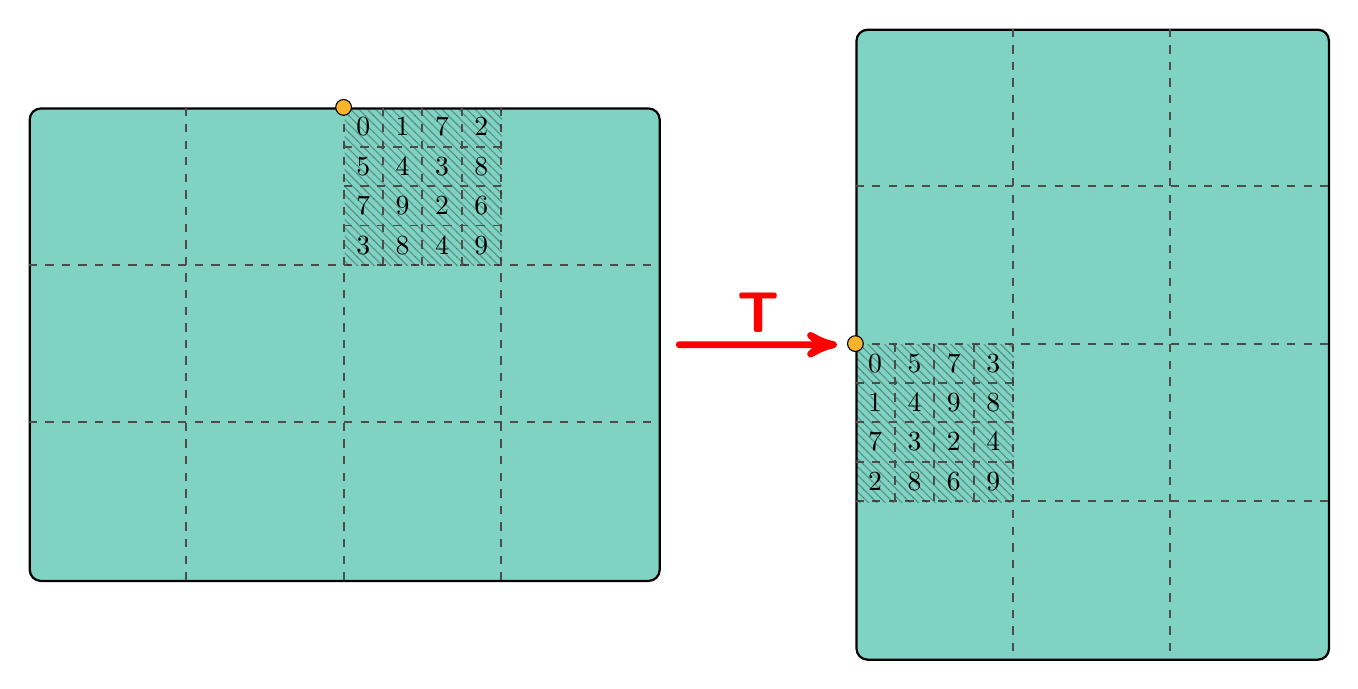
\begin{tikzpicture}[scale=1.0,transform shape]

  % Parameters
  \def\xcell{2.0cm}
  \def\ycell{2.0cm}

  % Styles
  \tikzstyle{table}=[draw,anchor=north west,thick,rounded corners]
  \tikzstyle{line}=[dashed,line width=0.7pt]
  \tikzstyle{to}=[->,>=stealth',shorten <=1pt,shorten >=1pt,line width=2.5pt,red,cap=round]

  % \table*{<id>}{<pos>}{<x-dim>}{<y-dim>}{<cell-lalbel-list>}[<optional-arguments>]
  % The star (*) argument enables drawing of lines between the cells
  \DeclareDocumentCommand \table { s m m m m m O{} }{%
    \path #3 node[table,minimum width=#4*\xcell,minimum height=#5*\ycell,#7] (table-#2) {};
    \IfBooleanT{#1}{%
      \pgfmathsetmacro\xdim{#4-1}
      \pgfmathsetmacro\ydim{#5-1}
      \ifnumgreater{#5}{1}{%
        \foreach \y in {1,...,\ydim}
          \draw[line,Black!70] ($(table-#2.north west)+(0,-\y*\ycell)$) -- ++(#4*\xcell,0);}{}
      \ifnumgreater{#4}{1}{%
        \foreach \x in {1,...,\xdim}
          \draw[line,Black!70] ($(table-#2.north west)+(\x*\xcell,0)$) -- ++(0,-#5*\ycell);}{}
    }
    \foreach[count=\li from 0] \l in {#6}{%
      \pgfmathsetmacro\lx{mod(\li,#4) + 0.5}
      \pgfmathsetmacro\ly{int(\li/#4) + 0.5}
      \node (cell-label-#2-\li) at ($(table-#2.north west)+(\lx*\xcell,-\ly*\ycell)$) {\l};
    }
  }

  % ===========================================================================
 
  % Draw tables
  \table*{0}{(0,0)}{4}{3}{}[fill=Emerald!50]
  \table*{1}{(10.5cm,0.5*\ycell)}{3}{4}{}[fill=Emerald!50]

  % Draw tiles
  \def\xcell{0.5cm}
  \def\ycell{0.5cm}
  \table*{2}{($(table-0.north west)+(8*\xcell,0)$)}{4}{4}{$0$,$1$,$7$,$2$,$5$,$4$,$3$,$8$,$7$,$9$,$2$,$6$,$3$,$8$,$4$,$9$}[draw=none,sharp corners,pattern=north west lines,opacity=0.3]
  \table*{3}{($(table-1.north west)+(0,-8*\ycell)$)}{4}{4}{$0$,$5$,$7$,$3$,$1$,$4$,$9$,$8$,$7$,$3$,$2$,$4$,$2$,$8$,$6$,$9$}[draw=none,sharp corners,pattern=north west lines,opacity=0.3]

  % Draw reference points
  \draw[draw,fill=Dandelion] ($(table-0.north west)+(8*\xcell,0)$) circle (1mm);
  \draw[draw,fill=Dandelion] ($(table-1.north west)+(0,-8*\ycell)$) circle (1mm);

  % Draw transition arrow
  \draw[to] ($(table-0.east)+(2mm,0)$) -- node[midway,above] {\sffamily\huge\bfseries T} ($(table-1.west)+(-2mm,0)$);

\end{tikzpicture}
\caption{Representation of transpose.}
\label{fig:transpose}
\end{figure}

\clearpage
%!TEX root = ../main.tex

\begin{figure}[p]
\centering
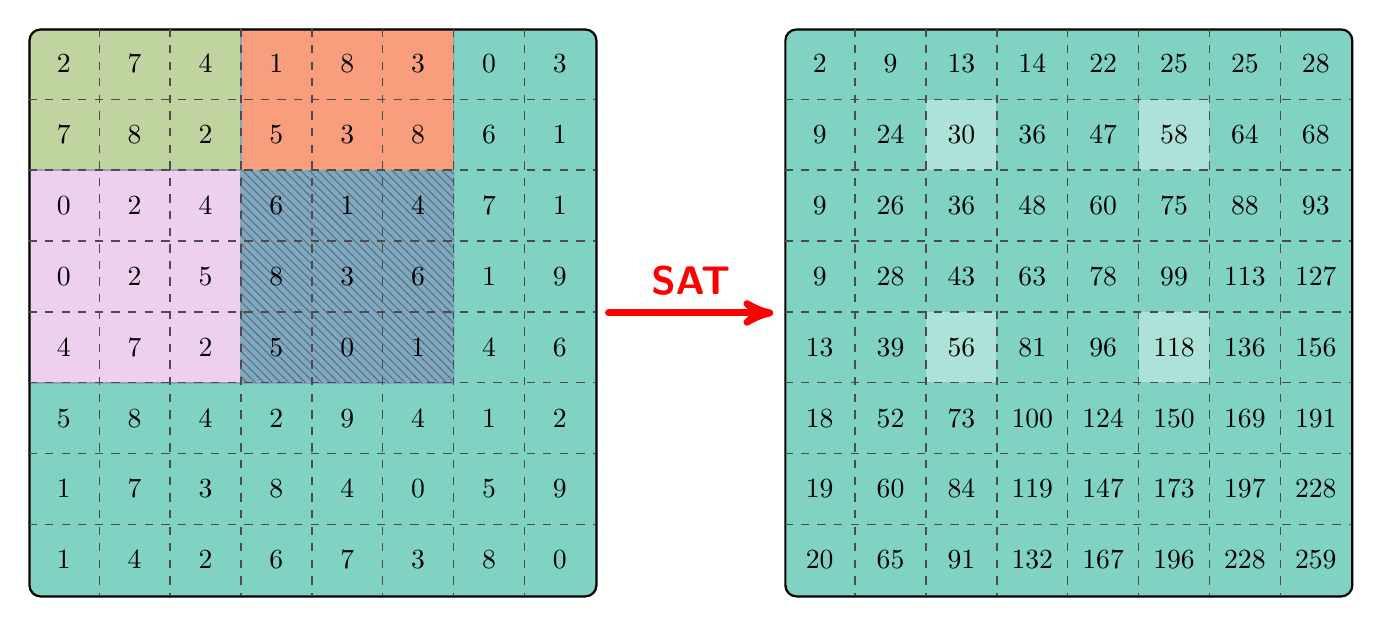
\begin{tikzpicture}[scale=1.0,transform shape]

  % Parameters
  \def\xcell{0.9cm}
  \def\ycell{0.9cm}
  \def\satshift{9.6cm}

  % Styles
  \tikzstyle{table}=[draw,anchor=north west,thick,rounded corners]
  \tikzstyle{line}=[dashed,line width=0.5pt]
  \tikzstyle{to}=[->,>=stealth',shorten <=4pt,shorten >=4pt,line width=2.5pt,red,cap=round]

  % \table*{<id>}{<pos>}{<x-dim>}{<y-dim>}{<cell-lalbel-list>}[<optional-arguments>]
  % The star (*) argument enables drawing of lines between the cells
  \DeclareDocumentCommand \table { s m m m m m O{} }{%
    \path #3 node[table,minimum width=#4*\xcell,minimum height=#5*\ycell,#7] (table-#2) {};
    \IfBooleanT{#1}{%
      \pgfmathsetmacro\xdim{#4-1}
      \pgfmathsetmacro\ydim{#5-1}
      \ifnumgreater{#5}{1}{%
        \foreach \y in {1,...,\ydim}
          \draw[line,Black!70] ($(table-#2.north west)+(0,-\y*\ycell)$) -- ++(#4*\xcell,0);}{}
      \ifnumgreater{#4}{1}{%
        \foreach \x in {1,...,\xdim}
          \draw[line,Black!70] ($(table-#2.north west)+(\x*\xcell,0)$) -- ++(0,-#5*\ycell);}{}
    }
    \foreach[count=\li from 0] \l in {#6}{%
      \pgfmathsetmacro\lx{mod(\li,#4) + 0.5}
      \pgfmathsetmacro\ly{int(\li/#4) + 0.5}
      \node (cell-label-#2-\li) at ($(table-#2.north west)+(\lx*\xcell,-\ly*\ycell)$) {\l};
    }
  }

  % ===========================================================================

  % Input array =================================
  
  % Draw background
  \table{0}{(0,0)}{8}{8}{}[draw=none,fill=Emerald!50]
  % Draw areas of interest
  \table{1}{(0,0)}{6}{5}{}[draw=none,xscale=0.997,yscale=0.997,append after command={\pgfextra \draw[draw=none,fill=NavyBlue!50,opacity=0.5] (\tikzlastnode.north) [rounded corners=0pt] -| (\tikzlastnode.east) [rounded corners=0pt] |- (\tikzlastnode.south) [rounded corners=0pt] -| (\tikzlastnode.west) [rounded corners=5pt] |- (\tikzlastnode.north); \endpgfextra}]
  \table{2}{(0,0)}{3}{2}{}[draw=none,xscale=0.985,yscale=0.978,append after command={\pgfextra \draw[draw=none,fill=Yellow!50,opacity=0.5] (\tikzlastnode.north) [rounded corners=0pt] -| (\tikzlastnode.east) [rounded corners=0pt] |- (\tikzlastnode.south) [rounded corners=0pt] -| (\tikzlastnode.west) [rounded corners=5pt] |- (\tikzlastnode.north); \endpgfextra}]
  \table{3}{(3*\xcell,0)}{3}{2}{}[draw=none,sharp corners,xscale=0.99,yscale=0.99,fill=RedOrange!50]
  \table{4}{(0,-2*\ycell)}{3}{3}{}[draw=none,sharp corners,xscale=0.99,yscale=0.99,fill=Plum!50]
  \draw[draw=none,pattern=north west lines,opacity=0.3] (3*\xcell,-2*\ycell) rectangle ++(3*\xcell,-3*\ycell);
  % Draw table of numbers
  \table*{5}{(0,0)}{8}{8}{$2$,$7$,$4$,$1$,$8$,$3$,$0$,$3$,$7$,$8$,$2$,$5$,$3$,$8$,$6$,$1$,$0$,$2$,$4$,$6$,$1$,$4$,$7$,$1$,$0$,$2$,$5$,$8$,$3$,$6$,$1$,$9$,$4$,$7$,$2$,$5$,$0$,$1$,$4$,$6$,$5$,$8$,$4$,$2$,$9$,$4$,$1$,$2$,$1$,$7$,$3$,$8$,$4$,$0$,$5$,$9$,$1$,$4$,$2$,$6$,$7$,$3$,$8$,$0$}

  % Summed area table ===========================

  % Draw background
  \table{6}{(\satshift,0)}{8}{8}{}[draw=none,fill=Emerald!50]
  % Draw cells of interest
  \table{11}{(\satshift+2*\xcell,-1*\ycell)}{1}{1}{}[draw=none,sharp corners,shift={(-0.01,0.01)},scale=0.99,fill=White,opacity=0.35]
  \table{12}{(\satshift+5*\xcell,-1*\ycell)}{1}{1}{}[draw=none,sharp corners,shift={(-0.01,0.01)},scale=0.99,fill=White,opacity=0.35]
  \table{13}{(\satshift+2*\xcell,-4*\ycell)}{1}{1}{}[draw=none,sharp corners,shift={(-0.01,0.01)},scale=0.99,fill=White,opacity=0.35]
  \table{14}{(\satshift+5*\xcell,-4*\ycell)}{1}{1}{}[draw=none,sharp corners,shift={(-0.01,0.01)},scale=0.99,fill=White,opacity=0.35]
  % Draw table of numbers
  \table*{15}{(\satshift,0)}{8}{8}{$2$,$9$,$13$,$14$,$22$,$25$,$25$,$28$,$9$,$24$,$30$,$36$,$47$,$58$,$64$,$68$,$9$,$26$,$36$,$48$,$60$,$75$,$88$,$93$,$9$,$28$,$43$,$63$,$78$,$99$,$113$,$127$,$13$,$39$,$56$,$81$,$96$,$118$,$136$,$156$,$18$,$52$,$73$,$100$,$124$,$150$,$169$,$191$,$19$,$60$,$84$,$119$,$147$,$173$,$197$,$228$,$20$,$65$,$91$,$132$,$167$,$196$,$228$,$259$}

  % Draw transition line
  \draw[to] (table-5.east) -- node[above,yshift=2] {\sffamily\bfseries\Large SAT} (table-15.west);

\end{tikzpicture}
\caption{Representation of a SAT application.}
\label{fig:sat}
\end{figure}

\clearpage
%!TEX root = ../main.tex

\begin{figure}[p]
\centering
\begin{tikzpicture}[scale=1.0,transform shape]

  % Definitions
  \newcommand*\rfrac[2]{{}^{#1}\!/_{#2}}

  % Layers
  \pgfdeclarelayer{next}
  \pgfsetlayers{main,next}

  % Parameters
  \def\dx{5cm}
  \def\dy{-0.7cm}
  \def\celldim{0.875cm}

  % Styles
  \tikzstyle{table}=[draw,anchor=north west,thick,opacity=0.8]
  \tikzstyle{line}=[dashed,line width=0.5pt]

  % \table{<id>}{<pos>}{<x-dim>}{<y-dim>}{<cell-label-list>}{<fill-color>}
  \DeclareDocumentCommand \table { m m m m m m }{%
    \path #2 node[table,fill=#6,minimum width=#3*\celldim,minimum height=#4*\celldim] (table-#1) {};
    \foreach \tmp [evaluate={\tmp-1} as \y] in {2,3,...,#3}
      \draw[line,Black!70] ($(table-#1.north west)+(0,-\y*\celldim)$) -- ++(#3*\celldim,0);
    \foreach \tmp [evaluate={\tmp-1} as \x] in {2,3,...,#4}
      \draw[line,Black!70] ($(table-#1.north west)+(\x*\celldim,0)$) -- ++(0,-#4*\celldim);
    \foreach[count=\li from 0] \l in {#5}
    {
      \pgfmathsetmacro\lx{mod(\li,#3) + 0.5}
      \pgfmathsetmacro\ly{int(\li/#3) + 0.5}
      \node (cell-label-#1-\li) at ($(table-#1.north west)+(\lx*\celldim,-\ly*\celldim)$) {\l};
    }
  }

  % ===========================================================================
 
  % Draw input image
  \pgftransformcm{0.7}{0.09}{-0.01}{1}{\pgfpoint{0cm}{0cm}}
  \node[anchor=north west,inner sep=0pt] (lena) at (0,0) {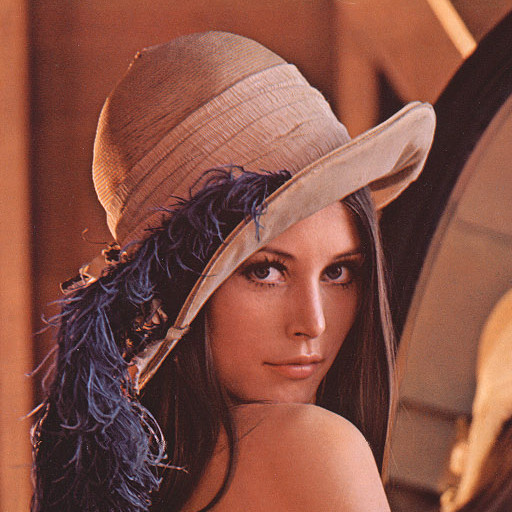
\includegraphics[width=7cm]{lena}};

  % Draw lines : input image -> input table
  \foreach \ref in {north west,north east,south west,south east}
    \draw[line] (lena.\ref) -- ++(\dx,\dy);

  % Draw input table
  \pgftransformcm{1}{0}{0}{1}{\pgfpoint{\dx}{\dy}}
  \node[table,fill=Cyan!50,minimum width=3*\celldim,minimum height=3*\celldim] at (0,0) {}; % Window
  \table{0}{(0,0)}{8}{8}{$2$,$7$,$4$,$1$,$8$,$3$,$0$,$3$,$7$,$8$,$2$,$5$,$3$,$8$,$6$,$1$,$0$,$2$,$4$,$6$,$1$,$4$,$7$,$1$,$0$,$2$,$5$,$8$,$3$,$6$,$1$,$9$,$4$,$7$,$2$,$5$,$0$,$1$,$4$,$6$,$5$,$8$,$4$,$2$,$9$,$4$,$1$,$2$,$1$,$7$,$3$,$8$,$4$,$0$,$5$,$9$,$1$,$4$,$2$,$6$,$7$,$3$,$8$,$0$}{LimeGreen!40}
  
  \begin{pgfonlayer}{next}
    % Draw filter kernel
    \pgftransformcm{1}{0}{0}{1}{\pgfpoint{\dx}{\dy}}
    \table{1}{(0,0)}{3}{3}{$\rfrac{1}{9}$,$\rfrac{1}{9}$,$\rfrac{1}{9}$,$\rfrac{1}{9}$,$\rfrac{1}{9}$,$\rfrac{1}{9}$,$\rfrac{1}{9}$,$\rfrac{1}{9}$,$\rfrac{1}{9}$}{RedOrange!40}

    % Draw output pixel lines
    \foreach \ref/\x/\y in {north west/1/1,north east/-1/1,south west/1/-1,south east/-1/-1}
      \draw[line] ($(table-1.\ref)$) -- ++(0.75*\dx+\x*\celldim,0.75*\dy-\y*\celldim);

    % Draw output table
    \pgftransformcm{1}{0}{0}{1}{\pgfpoint{0.75*\dx}{0.75*\dy}}
    \node[table,fill=RedOrange!55,minimum width=\celldim,minimum height=\celldim] at (\celldim,-\celldim) {}; % pixel
    \table{2}{(0,0)}{8}{8}{$3$,$3$,$3$,$3$,$3$,$3$,$2$,$1$,$3$,$4$,$4$,$4$,$4$,$4$,$4$,$2$,$2$,$3$,$5$,$4$,$5$,$4$,$5$,$3$,$2$,$3$,$5$,$4$,$4$,$3$,$4$,$3$,$3$,$4$,$5$,$4$,$4$,$3$,$4$,$3$,$4$,$5$,$5$,$4$,$4$,$3$,$4$,$3$,$3$,$4$,$5$,$5$,$5$,$5$,$4$,$3$,$1$,$2$,$3$,$3$,$3$,$3$,$3$,$2$}{Goldenrod!40}

    % Draw lines : output table -> output image
    \foreach \ref in {north west,north east,south west,south east}
      \draw[line] (table-2.\ref) -- ++(\dx,\dy);

    % Draw output image
    \pgftransformcm{1}{0}{0}{1}{\pgfpoint{\dx}{\dy}}
    \node[anchor=north west,inner sep=0pt] (lena-filtered) at (0,0) {
\includegraphics[width=7cm]{lena-filtered}};
  \end{pgfonlayer}

  % Draw lines : input table -> filter kernel
  \foreach \ref in {north west,north east,south west,south east}
    \draw[line] (table-1.\ref) -- ++(-\dx,-\dy);

  % Draw labels
  \node[above] at (table-0.north east) {\sffamily\Large input};
  \node[above] at (table-1.north east) {\sffamily\Large filter};
  \node[above] at (table-2.north east) {\sffamily\Large output};

\end{tikzpicture}
\caption{Representation of box filter.}
\label{fig:box-filter}
\end{figure}

\clearpage
%!TEX root = ../main.tex

\begin{figure}[p]
\centering
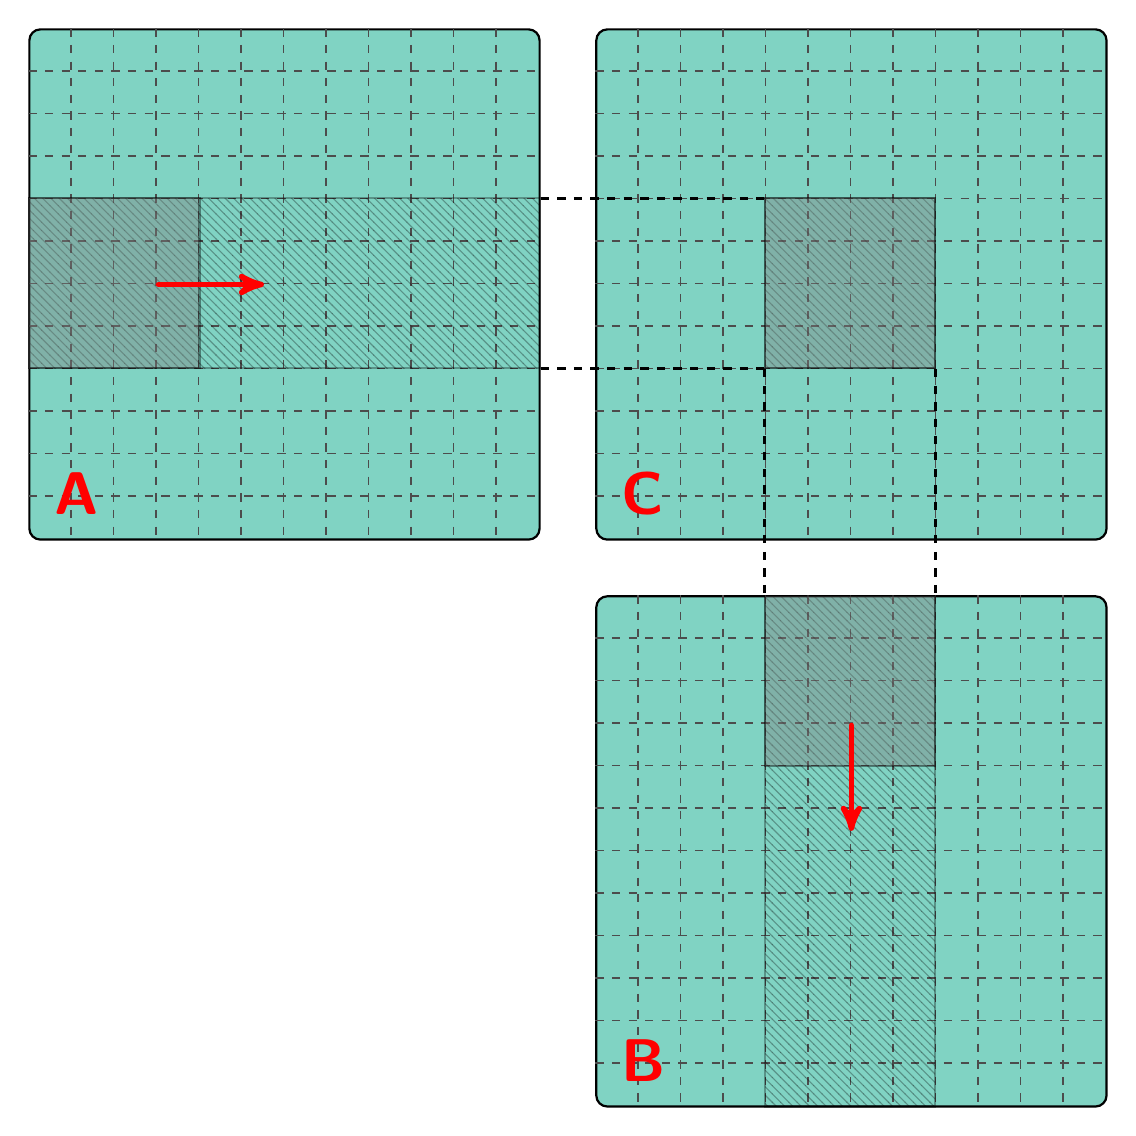
\begin{tikzpicture}[scale=0.9,transform shape]

  % Parameters
  \def\xcell{0.6cm}
  \def\ycell{0.6cm}
  \def\tabshift{8cm}

  % Styles
  \tikzstyle{table}=[draw,anchor=north west,thick,rounded corners]
  \tikzstyle{shade-lines}=[draw,thick,anchor=north west,fill=gray,opacity=0.3,pattern=north west lines,text centered]
  \tikzstyle{shade-fill}=[draw,thick,anchor=north west,fill=gray,opacity=0.3,text centered]
  \tikzstyle{line}=[dashed,line width=0.5pt]
  \tikzstyle{to}=[->,>=stealth',shorten <=4pt,shorten >=4pt,line width=2pt,Red,cap=round]

  % \table*{<id>}{<pos>}{<x-dim>}{<y-dim>}{<cell-lalbel-list>}[<optional-arguments>]
  % The star (*) argument enables drawing of lines between the cells
  \DeclareDocumentCommand \table { s m m m m m O{} }{%
    \path #3 node[table,minimum width=#4*\xcell,minimum height=#5*\ycell,#7] (table-#2) {};
    \IfBooleanT{#1}{%
      \pgfmathsetmacro\xdim{#4-1}
      \pgfmathsetmacro\ydim{#5-1}
      \ifnumgreater{#5}{1}{%
        \foreach \y in {1,...,\ydim}
          \draw[line,Black!70] ($(table-#2.north west)+(0,-\y*\ycell)$) -- ++(#4*\xcell,0);}{}
      \ifnumgreater{#4}{1}{%
        \foreach \x in {1,...,\xdim}
          \draw[line,Black!70] ($(table-#2.north west)+(\x*\xcell,0)$) -- ++(0,-#5*\ycell);}{}
    }
    \foreach[count=\li from 0] \l in {#6}{%
      \pgfmathsetmacro\lx{mod(\li,#4) + 0.5}
      \pgfmathsetmacro\ly{int(\li/#4) + 0.5}
      \node (cell-label-#2-\li) at ($(table-#2.north west)+(\lx*\xcell,-\ly*\ycell)$) {\l};
    }
  }

  % \shade*{<id>}{<pos>}{<x-cells>}{<y-cells>}[<optional-arguments>]
  % The star (*) argument chooses a shading style
  \DeclareDocumentCommand \shade { s m m m m O{} }{%
    \path #3 node[\IfBooleanTF{#1}{shade-fill}{shade-lines},minimum width=#4*\xcell,minimum height=#5*\ycell,#6] (shade-#2) {};
  }

  % ===========================================================================

  % Draw tables
  \table*{0}{(0,0)}{12}{12}{}[fill=Emerald!50]
  \table*{1}{(\tabshift,0)}{12}{12}{}[fill=Emerald!50]
  \table*{2}{(\tabshift,-\tabshift)}{12}{12}{}[fill=Emerald!50]

  % Draw shades
  \shade{0}{($(table-0.north west)+(0,-4*\ycell+0.2mm)$)}{12}{4}
  \shade{1}{($(table-1.north west)+(4*\xcell-0.2mm,-4*\ycell+0.2mm)$)}{4}{4}
  \shade{2}{($(table-2.north west)+(4*\xcell-0.2mm,0)$)}{4}{12}
  \shade*{3}{($(table-0.north west)+(0,-4*\ycell+0.2mm)$)}{4}{4}[opacity=0.4]
  \shade*{4}{($(table-1.north west)+(4*\xcell-0.2mm,-4*\ycell+0.2mm)$)}{4}{4}[opacity=0.4]
  \shade*{5}{($(table-2.north west)+(4*\xcell-0.2mm,0)$)}{4}{4}[opacity=0.4]

  % Draw support lines
  \draw[line,line width=1.1pt] ($(shade-0.north east)+(0,-0.2mm)$) -- ($(shade-4.north west)+(0,-0.2mm)$);
  \draw[line,line width=1.1pt] ($(shade-0.south east)+(0,0.1mm)$) -- ($(shade-4.south west)+(0,0.1mm)$);
  \draw[line,line width=1.1pt] ($(shade-4.south west)+(0.1mm,0)$) -- ($(shade-2.north west)+(0.1mm,0)$);
  \draw[line,line width=1.1pt] ($(shade-4.south east)+(-0.1mm,0)$) -- ($(shade-2.north east)+(-0.1mm,0)$);

  % Draw arrows
  \draw[to] ($(table-0.west)+(2.8*\xcell,0)$) -- ++(3*\xcell,0);
  \draw[to] ($(table-2.north)+(0,-2.8*\ycell)$) -- ++(0,-3*\ycell);

  % Draw labels
  \node[above right,shift={(2mm,2mm)},scale=1.4,Red] at (table-0.south west) {\sffamily\bfseries\LARGE A};
  \node[above right,shift={(2mm,2mm)},scale=1.4,Red] at (table-2.south west) {\sffamily\bfseries\LARGE B};
  \node[above right,shift={(2mm,2mm)},scale=1.4,Red] at (table-1.south west) {\sffamily\bfseries\LARGE C};

\end{tikzpicture}
\caption{Representation of matrix-matrix multiplication.}
\label{fig:mat-mat-mult}
\end{figure}

\clearpage

\end{document} 
